% =========================================================================
% Distributed Observability for Multi-Agent LLM Systems:
% A Shared-Log Approach on HPC Clusters
%
% Build: pdflatex main && bibtex main && pdflatex main && pdflatex main
% (or just upload the thesis/ folder to Overleaf)
% =========================================================================
\documentclass[11pt,a4paper]{report}

\usepackage[utf8]{inputenc}
\usepackage[T1]{fontenc}
\usepackage[english]{babel}
\usepackage{graphicx}
\usepackage{booktabs}
\usepackage{amsmath}           % \text{} in the complexity expressions
\usepackage{amssymb}           % \checkmark in the substrate feature matrix
\usepackage{tikz}
\usetikzlibrary{arrows.meta, positioning, fit, decorations.pathreplacing}
\usepackage{pgfplots}          % measured-data plots (e.g. fig-rollup-scaling)
\pgfplotsset{compat=1.17}
% One visual language for every measured-data plot. The default pgfplots cycle
% is blue/red, which made the five evaluation figures look like three unrelated
% documents and reproduces poorly in print; this greyscale cycle plus a
% recessive grid and legend is applied document-wide so the figures read as one
% system. Bar charts set their fills explicitly and use \addplot (not
% \addplot+), so no cycle colour leaks into their value labels.
\pgfplotsset{
  cycle list={%
    {black!75, mark=*, mark size=1.6pt, mark options={fill=black!30, draw=black!75}},%
    {black!45, mark=square*, mark size=1.6pt, mark options={fill=black!8, draw=black!45}},%
  },
  every axis/.append style={
    grid=major,
    grid style={dashed, gray!25},
    tick style={draw=gray!50},
    legend cell align=left,
    legend style={font=\small, draw=gray!40},
  },
}
\usepackage{microtype}
\usepackage[margin=2.45cm]{geometry}
% The report class reserves ~2 inches of whitespace above every chapter
% title; with 11 chapter-level headings that is most of a page. Tighten it.
% Default float rules reserve 20% of any float page for text, which strands a
% lone screenshot on a page of its own. Let figures pack together instead.
\renewcommand{\topfraction}{0.92}
\renewcommand{\bottomfraction}{0.92}
\renewcommand{\textfraction}{0.06}
\renewcommand{\floatpagefraction}{0.82}
% The captions in this document are long and numerous (25 floats); setting them
% one size down and tightening float separation recovers several pages without
% touching a word of the prose or the 2.6cm margins the template fixes.
\usepackage[font=small,labelfont=bf,skip=5pt]{caption}
% The contents ran 250 characters past a page boundary, claiming a second page
% for three lines. Tightening the gap the TOC leaves before each chapter block
% recovers it without dropping the section level, which is worth keeping.
\usepackage{tocloft}
\setlength{\cftbeforechapskip}{2pt}
\setlength{\textfloatsep}{10pt plus 2pt minus 3pt}
\setlength{\intextsep}{10pt plus 2pt minus 3pt}
\setlength{\dbltextfloatsep}{10pt plus 2pt minus 3pt}
\usepackage{titlesec}
\titleformat{\chapter}[display]
  {\normalfont\huge\bfseries}{\chaptertitlename\ \thechapter}{10pt}{\Huge}
\titlespacing*{\chapter}{0pt}{-20pt}{24pt}
% Lets TeX stretch a problem line rather than overflow the margin; the
% prose carries many unbreakable \texttt{} identifiers.
\emergencystretch=3em
% `hyphens' lets long URLs in the bibliography break across lines.
\PassOptionsToPackage{hyphens}{url}
\usepackage[hidelinks]{hyperref}

% Placeholder for numbers not yet measured — grep for \tbd before submission.
\newcommand{\tbd}[1]{\textbf{[TBD: #1]}}
% Support levels in the substrate feature matrix (Table 3.4). Named with a
% leading f so \fpart cannot collide with LaTeX's \part sectioning command.
\newcommand{\fyes}{\ensuremath{\checkmark}}
\newcommand{\fpart}{\ensuremath{\circ}}
\newcommand{\fno}{\ensuremath{\times}}

\begin{document}

% ------------------------------ Title page -------------------------------
% Hand-built rather than \maketitle: the default report title block cannot
% carry the institution or the advisor line.
\begin{titlepage}
\centering
\vspace*{\stretch{1}}

{\LARGE\bfseries Distributed Observability for\\[0.35em]
 Multi-Agent LLM Systems\par}

\vspace{0.9em}
{\large A Shared-Log Approach on HPC Clusters\par}

\vspace{1.6em}
\rule{0.62\linewidth}{0.4pt}\par
\vspace{1.1em}
{\small An observability framework for LLM-agent fleets on HPC clusters\par}
\vspace{1.1em}
\rule{0.62\linewidth}{0.4pt}\par

\vspace{\stretch{1.1}}

{\large\bfseries Anna Mons\'o Rodriguez\par}
\vspace{0.25em}
{\small A20653296\par}

\vspace{1.8em}
{\small Advisor: Jaime Cernuda\par}

\vspace{\stretch{1.2}}

{\large Illinois Institute of Technology\par}
\vspace{0.3em}
{\small Chicago, Illinois\par}
\vspace{1.2em}
{\small \today\par}

\vspace*{\stretch{0.6}}
\end{titlepage}

\begin{abstract}
Applications built on large language models (LLMs) have outgrown the tooling
built to observe them. They have changed in two ways at once: they have
become multi-agent, and they have moved onto clusters.
Observability tooling has followed one change or the other, never both:
LLM-observability platforms capture rich agent semantics but have no notion
of the physical machines involved, while HPC and fleet monitoring tracks
node health at scale but carries no application semantics. To our
knowledge, no existing tool spans the two.

This thesis begins from the observation that a multi-agent execution is
already a causally-ordered event log, and tests the hypothesis that follows:
if such a fleet's events are captured into a distributed shared log whose
store places an append endpoint on every compute node, then agent semantics
and cluster topology are coupled by construction, and a single reader over
that log can answer the operator's fleet-scale questions.

To keep the design independent of any one store, we state the contract a
store must honour: five required features (caller-named, ordered, durable,
replayable, multi-reader streams) and four convenient ones whose absence
costs a named mechanism rather than a redesign. Against that contract we
design an observability framework for LLM-agent fleets, and implement
it on ChronoLog, a distributed tiered log store that runs a capture process
on every cluster node. Two capture paths feed the log (LLM turns through
a node-local spool drained by a capture worker, inter-agent calls through
per-node collectors), with at-least-once capture and effectively
exactly-once ingest. Because that log is optimized for ingest and cannot be
read inside its acceptance window, a hot/cold read design serves real-time
views from the same event stream. On top of it we build fleet-scale
analyses: failure detection that groups textually identical failures into
ranked, diagnosed incidents at no token cost; per-node health rollups whose
cost is independent of event volume; and cross-host critical-path tracing.

We validate the system end to end with real Claude agents on live 4- and
8-node ChronoLog clusters, passing 28 of 28 automated checks with up to 32
concurrent agents, and measure it throughout. Capture costs an agent
3.6\,ms per turn, statistically invisible against real LLM latency. Events
reach the operator's screen in 10.7\,ms, against a 20--30\,s durable drain.
Fleet queries stay flat as event volume grows $50\times$. A ground-truth
fault study scores 580 of 580 detections with zero false positives. In a
timed case study, a first-time operator produced a complete, verified
cross-layer diagnosis in 72 seconds, a task they could not begin from the
raw logs. The implementation is a research prototype: it is validated at
the scales reported here, and its limits are stated alongside the results.
\end{abstract}

% Sections only: the subsection level pushed the contents onto a second page
% without helping a reader navigate a document this size.
\setcounter{tocdepth}{1}
\tableofcontents
% The figure and table lists are short enough to share a page; suppressing the
% \clearpage that \chapter* issues lets the second follow the first instead of
% claiming a page of its own.
\listoffigures
\begingroup\let\clearpage\relax\listoftables\endgroup

% Runs on from the list of tables rather than claiming a page of its own.
\section*{Acronyms}
\begin{tabular}{@{}ll@{\hspace{2.2em}}ll@{}}
LLM  & Large Language Model            & JSONL& JSON Lines \\
MCP  & Model Context Protocol          & CSV  & Comma-Separated Values \\
HPC  & High-Performance Computing      & HDF5 & Hierarchical Data Format, v5 \\
SLURM& Simple Linux Utility for        & p95  & 95th percentile \\
     & \quad Resource Management       & RSS  & Resident Set Size \\
SSE  & Server-Sent Events              & APM  & Application Performance Monitoring \\
API  & Application Programming Interface & eBPF & extended Berkeley Packet Filter \\
SDK  & Software Development Kit        & DNS  & Domain Name System \\
GIL  & Global Interpreter Lock         & UI   & User Interface \\
NFS  & Network File System             & RPC  & Remote Procedure Call \\
\end{tabular}

% ------------------------------- Chapters --------------------------------
\chapter{Introduction}
\label{chap:intro}

This chapter motivates the thesis: it describes the workload (fleets
of LLM agents on HPC clusters) and the observability gap it creates,
states the observation the design builds on, and lists the
contributions and the document structure.

\section{Context: Multi-Agent LLM Systems on Clusters}
\label{sec:intro-context}

Applications built on large language models (LLMs) have changed shape
quickly over the last few years. The first generation consisted of single
request--response calls: a prompt in, a completion out. The second generation
wrapped the model in a loop, the \emph{agent}, in which the model is
prompted with a task and a transcript, emits a call to an external tool,
has the tool's result appended to that transcript, and is prompted again,
until it emits a final answer instead of a call~\cite{yao2023react}.
Section~\ref{sec:bg-agent-loop} gives the mechanism precisely; the term
\emph{agent} is used throughout this thesis for that loop and the process
running it, and for nothing more. The current generation
goes one step further and decomposes a task across \emph{multiple}
cooperating agents, each with its own role, context, and
conversation, which delegate sub-tasks to one another through structured
tool-call protocols such as the Model Context Protocol
(MCP)~\cite{anthropic2024mcp}. Multi-agent frameworks make this pattern
routine~\cite{wu2023autogen}: a planner agent delegates sub-tasks to worker
agents, workers consult specialist agents, and the overall computation is a
conversation \emph{between} programs as much as within them.

At the same time, the deployment platform of these systems is changing.
When agents were single processes, a laptop or a single cloud instance was
enough. Multi-agent workloads (scientific-workflow assistants, large-scale
code analysis, data-processing fleets) instead run on
\emph{clusters}: tens to hundreds of nodes, allocated through batch schedulers
such as SLURM~\cite{yoo2003slurm}, with several agents per node. Recent
work places LLM-agent orchestration directly on leadership-class HPC
systems~\cite{pham2026multiagenthpc} and on the workflow infrastructure
that spans them~\cite{souza2025provenance}. The result
is a genuinely distributed system in the classical sense: many processes on
many machines, communicating over a network, with no shared clock and no
single point of observation.

This combination is operationally demanding in a way neither ancestor was.
LLM agents are non-deterministic, expensive (every turn has a token cost),
slow (seconds per model call), and failure-prone in unfamiliar ways.
They retry, emit calls naming tools or arguments that do not exist, hang on
remote calls, and
silently degrade; empirical studies of multi-agent LLM systems find such
failures to be systematic rather than incidental~\cite{cemri2025mast}, and
the retry loops in particular are an instance of the amplification
pathologies long known to destabilize distributed
systems~\cite{bronson2021metastable}.
Running \emph{fleets} of them across a cluster multiplies these problems by
the number of nodes and adds the classical failure modes of distributed
infrastructure: slow nodes, network partitions, and stragglers that drag
down the whole computation~\cite{gunawi2018failslow}. An operator
needs to answer questions that span both layers at once: \emph{What is
the fleet doing right now? Which agents are talking to which? Why is this
scenario slow, and which hop is the bottleneck? Which node is dragging the
fleet down? Has this failure happened before?}

This setting is the object of study of this thesis: a fleet of LLM
agents distributed across the nodes of a high-performance-computing (HPC)
cluster, and the observability infrastructure required to operate it.

\section{The Gap: Agent Semantics vs.\ Cluster Topology}
\label{sec:intro-gap}

Observability tooling for this setting splits into two mature camps whose
intersection is, to our knowledge, unoccupied. The first camp,
\emph{LLM and agent observability} (LangSmith~\cite{langsmith},
Langfuse~\cite{langfuse}, Arize Phoenix~\cite{phoenix},
AgentOps~\cite{agentops}, the LLM products of established APM
vendors~\cite{datadogllm}, and the OpenTelemetry generative-AI semantic
conventions now consolidating them~\cite{otelgenai}), captures rich agent
semantics (prompts, tokens, costs, tool calls, rendered as traces of nested
spans in the lineage of Dapper~\cite{sigelman2010dapper}) but treats
the physical machines the agents run on as, at best, opaque metadata: host
identity is not a dimension the tools can group, compare, or alert over.
The second camp, \emph{HPC and fleet monitoring}
(Prometheus~\cite{prometheus} with Grafana over batch-scheduled clusters, and
HPC-native collectors such as LDMS~\cite{agelastos2014ldms}), is built for
that physical layer (per-node metrics at scale, over hundreds of
nodes) but carries no application semantics at all: that the process
saturating a node is an LLM agent mid-conversation, retrying a failed
delegation, is invisible. Section~\ref{sec:bg-sota} surveys both camps in
detail.

The consequence fits in one sentence, which this thesis takes as its
motivating problem:

\begin{quote}
\emph{The tools we survey answer ``what did my agent do?'' with a trace
of one run on one machine. To our knowledge, none answers ``what is
my agent \textbf{fleet} doing across the cluster, and which node is
dragging it down?''}
\end{quote}

Answering that question requires coupling agent semantics to physical
cluster topology in a single system, the intersection both camps leave
open.

\section{The Log-Based Approach}
\label{sec:intro-insight}

The technical starting point is an observation about the shape
of the data. Everything worth capturing about a multi-agent system is an
\emph{event}: an LLM turn (prompt, response, tokens, latency, cost), an
agent-to-agent call (caller, callee, correlation, outcome), a
retained-context operation (an item added to or evicted from the material
an agent's next prompt is assembled from, \S\ref{sec:bg-agent-signals}), a
recovery or backtrack. These events carry timestamps and causal
relationships: a delegation \emph{happens before} the turns it triggers,
which happen before the reply edge. A multi-agent execution, in other words,
\emph{is} a causally-ordered event log in the sense of
Lamport~\cite{lamport1978time}.

If the data is natively a distributed event log, the natural place to store
it is a \emph{distributed shared log}~\cite{balakrishnan2012corfu,
kreps2013log}, the abstraction industrialized by Kafka~\cite{kreps2011kafka}
and since carried into production control planes~\cite{balakrishnan2020delos}.
This thesis uses the term \emph{substrate} for that storage
system: the log store underneath the observability system, whichever one it
is. Agents append locally on the node where they run; the log
provides ordering, durability, and archival; and every observability view is
a \emph{reader} over the same substrate. Ordering and durability become
properties of the storage layer rather than of the instrumentation, and
cross-agent causal reconstruction comes with the substrate rather than being
bolted on.

This yields the hypothesis the thesis tests: \emph{if the events of a
multi-agent LLM fleet are captured into a distributed shared log whose store
places an append endpoint on every compute node, then agent semantics and
cluster topology are coupled by construction rather than by integration, and
a reader over that one log can answer the operator's fleet-scale questions
without further instrumentation.} It is testable in two parts.
Section~\ref{sec:problem-substrate} makes the storage half checkable by
stating the features a store must provide, so that any candidate can be
scored against it; Chapter~\ref{chap:evaluation} measures the second half
against the requirements of \S\ref{sec:problem-requirements}.

Which store provides the log is a separate question, and this thesis keeps
it separate: \S\ref{sec:problem-substrate}
states the contract a substrate must honour (five required features,
S1--S5, and four convenient ones, S6--S9, each of whose absence is priced
in a named mechanism), and Chapter~\ref{chap:design} is written against
that contract. The implementation runs on
ChronoLog~\cite{kougkas2020chronolog}, a distributed, tiered shared-log
store that orders events by physical time and, crucially for this setting,
places a log-capture process (a \emph{keeper}) on every cluster node, so
that the mapping from an event to the machine that produced it is a fact
about where the append landed rather than a field the instrumentation must
be trusted to fill in. That property, S6 in the contract, is what no
general-purpose commit log offers and what makes the coupling of agent
semantics to cluster topology structural. Section~\ref{sec:design-chronolog}
reports the ChronoLog-specific consequences in one place, so that the design
and its instantiation can be read, and criticized, separately.

On this foundation the thesis designs, implements, and validates an
observability framework for LLM-agent fleets on HPC clusters. It
is a research prototype: complete enough to run real agent fleets on a
live cluster and to be measured end to end, but validated at the scales
reported in Chapter~\ref{chap:evaluation} rather than hardened for
production use.
Two capture paths feed the log,
one for LLM turns and one for inter-agent
calls, and a dashboard reconstructs every view (live agent and cluster
topology, failure diagnosis, fleet health, cross-host tracing) purely
from what was captured. Because a shared log of this class is
optimized for ingest (archive reads trail appends by tens of seconds of
drain latency, and on the deployed client a live replay can block a reader
for minutes), the
system adopts a two-path read design: the log is the
durable \emph{cold} path, and an in-process \emph{hot} store serves real-time
views from the same event stream at ingest time. That split is the price of
one feature the substrate contract marks optional, and
\S\ref{sec:design-adapters} says precisely what a store providing it would
let a reimplementation delete. We validate the system
end-to-end with real Claude agents on live multi-node ChronoLog deployments.

\section{Contributions}
\label{sec:intro-contributions}

This thesis makes five contributions:

\begin{enumerate}
\item \textbf{A substrate contract for log-backed observability.} We
  identify the minimal set of features a storage substrate must provide for
  an observability system of this shape to be implementable on it (S1--S5),
  together with a second tier (S6--S9) whose absence is survivable at a
  stated price, and we score representative shared logs against both
  (Chapter~\ref{chap:problem}). The contract is what makes the rest of the
  design portable rather than particular: it separates the architecture from
  the workarounds one deployment required, and it lets a prospective adopter
  predict the cost of a port from a table rather than discover it during one.
\item \textbf{A two-path capture architecture over a distributed shared log.}
  LLM turns flow through a node-local \emph{spool}, an append-only file on
  the agent's own machine, drained into the log by a separate
  \emph{capture worker} process; inter-agent calls flow through a per-node
  \emph{collector} daemon into that node's keeper. The design provides
  at-least-once capture and effectively exactly-once ingest, deduplicating
  on a per-session sequence number (a \emph{high-water mark}), with crash
  recovery reconstructed from the log itself (Chapter~\ref{chap:design}).
\item \textbf{A hot/cold read design around the log's ingest-optimized
  trade-off.} The log store's drain latency (tens of seconds) and a
  replay path that can block the reader for minutes make it
  unreadable in real time; the system pairs it with an in-process
  \emph{hot store} written at the moment of ingest, and a
  server-sent-events (SSE) \emph{live bus} that pushes each event on to the
  browser, so that real-time views and durable
  full-fidelity views are projections of one event stream
  (Chapter~\ref{chap:design}).
\item \textbf{Fleet-scale analytics computed on the log.} Three analyses turn
  the captured events into operator answers: a failure-diagnosis pipeline,
  the \emph{Doctor}, which detects
  failures, groups the textually identical ones into ranked incidents, and
  attaches zero-cost diagnoses with cross-run incident history; fleet-health
  \emph{rollups}, per-(host, minute) buckets aggregated at write time, that
  make the cluster overview $O(\mathrm{nodes}\times\mathrm{buckets})$,
  independent of event volume; and cross-host critical-path tracing that
  names the bottleneck hop by \emph{self-time}, its latency minus its
  slowest child's (Chapter~\ref{chap:analytics}).
\item \textbf{A measured evaluation on live clusters.} An automated
  end-to-end harness exercises the full stack with real Claude Agent SDK
  agents on live 4- and 8-node ChronoLog clusters, and we measure
  five dimensions: capture overhead, freshness, detection quality against
  planted ground truth, scalability in event volume and agent count, and
  a timed cross-layer diagnosis case study
  (Chapter~\ref{chap:evaluation}).
  Real agents provide the end-to-end ground truth; a synthetic generator
  driving the \emph{identical} ingest path supplies the controlled,
  reproducible load for the scale sweeps, where thousands of turns of real
  inference would be neither affordable nor repeatable
  (\S\ref{sec:eval-method}).
  Section~\ref{sec:eval-limitations} bounds each of those claims: the
  scales actually validated, the diagnoser's coverage, and the substrate
  behaviour the design works around rather than fixes.
\end{enumerate}

\section{Document Structure}
\label{sec:intro-structure}

Chapter~\ref{chap:background} develops the background (distributed-systems
foundations, distributed tracing, the shared-log abstraction, ChronoLog, and
LLM agents) and surveys the state of the art to establish the gap.
Chapter~\ref{chap:problem} distills the target scenario into explicit
requirements and states the substrate contract S1--S9. The system design
follows in Chapter~\ref{chap:design}: the
capture paths, the mapping of agent semantics onto the log, delivery
semantics, and the hot/cold read split, written against that contract, with
\S\ref{sec:design-chronolog} collecting what the ChronoLog instantiation
adds. Chapter~\ref{chap:analytics} builds
the fleet-scale analyses on top of it. Chapter~\ref{chap:evaluation}
measures overhead, freshness, scalability, and end-to-end correctness, and
closes with a fault-localization case study. Chapter~\ref{chap:conclusions}
concludes.

\chapter{Background and State of the Art}
\label{chap:background}

This chapter develops the concepts the thesis is built from, as a
progression: the distributed-systems fundamentals that define the
problem's vocabulary (\S\ref{sec:bg-ds}); distributed tracing, the discipline
that first made cross-machine causality observable
(\S\ref{sec:bg-tracing}); the distributed shared log, the storage abstraction
this thesis adopts as its substrate (\S\ref{sec:bg-log}); ChronoLog, the
concrete log store used (\S\ref{sec:bg-chronolog}); LLM agents and
multi-agent systems, the workload being observed (\S\ref{sec:bg-agents});
and finally the state of the art, whose two disjoint camps define the gap
this thesis targets (\S\ref{sec:bg-sota}). Most sections close by noting
what the thesis takes from them.

\section{Distributed Systems Fundamentals}
\label{sec:bg-ds}

\subsection{Time, Ordering, and Causality}
\label{sec:bg-time}

A distributed system is a set of processes on separate machines that
communicate only by exchanging messages. Its defining difficulty is that
there is no global ``now'': each machine has its own clock, clocks drift, and
no observer sees the whole system at once. Any statement about what the
system \emph{is doing} must therefore be reconstructed from locally
recorded observations.

Lamport's insight is that such reconstruction turns not on wall-clock
simultaneity but on \emph{causality}, captured by the
\emph{happened-before} relation~\cite{lamport1978time}: event $a$
happened before event $b$ if they occur in that order in the same process, or
if $a$ is the sending of a message that $b$ receives, or transitively through
a chain of such steps (Figure~\ref{fig:hb}). Happened-before is a partial
order (some event pairs are simply concurrent), and it is the order
that determines whether one event could have influenced another: in
Figure~\ref{fig:hb}, $a$ happened before $d$ through the chain
$a \to c \to e \to d$, while $b$ and $e$ are concurrent: no causal path
connects them, even though $b$ occurs later in wall-clock time.

\begin{figure}[t]
  \centering
  % Space-time diagram: happened-before, causal chains, concurrency.
\begin{tikzpicture}[>=Stealth, thick, font=\small]
  % process timelines
  \foreach \y/\p in {0/{$P_3$}, 1.5/{$P_2$}, 3.0/{$P_1$}} {%
    \draw[->, semithick] (0,\y) -- (10.4,\y);
    \node[left=3pt] at (0,\y) {\p};
  }
  \node[below right] at (9.4,-0.1) {\footnotesize wall-clock time};
  % events
  \filldraw (1.2,3.0) circle (2.2pt) node[above=2pt] {$a$};
  \filldraw (5.2,3.0) circle (2.2pt) node[above=2pt] {$b$};
  \filldraw (2.6,1.5) circle (2.2pt) node[above=2pt] {$c$};
  \filldraw (6.6,1.5) circle (2.2pt) node[above=2pt] {$d$};
  \filldraw (4.2,0)   circle (2.2pt) node[below=2pt] {$e$};
  \filldraw (8.6,0)   circle (2.2pt) node[below=2pt] {$f$};
  % messages
  \draw[->] (1.2,3.0) -- node[midway, left=2pt]  {\footnotesize $m_1$} (2.6,1.5);
  \draw[->] (2.6,1.5) -- node[midway, left=2pt]  {\footnotesize $m_2$} (4.2,0);
  \draw[->] (4.2,0)   -- node[midway, right=3pt] {\footnotesize $m_3$} (6.6,1.5);
\end{tikzpicture}

  \caption{A space-time diagram of three processes exchanging messages
  $m_1$--$m_3$. Causality flows along process lines and messages:
  $a \rightarrow c \rightarrow e \rightarrow d$ is a causal chain, so $a$
  \emph{happened before} $d$; $b$ and $e$ are \emph{concurrent} (neither
  could have influenced the other), despite $b$ being later on the wall
  clock.}
  \label{fig:hb}
\end{figure}

Logical and vector
clocks~\cite{lamport1978time,fidge1988timestamps,mattern1989virtual} make
this order computable
from local information; alternatively, when all events carry timestamps from
reasonably synchronized physical clocks and land in one ordered store, causal
chains follow from timestamps plus application-level correlation identifiers.

The corollary this thesis leans on is that the
\emph{event log}, an append-only sequence of timestamped, attributed
events, is the canonical representation of distributed execution. A log
captures exactly what each process observed and when; every richer structure
(a request trace, a communication graph, a health summary) is a fold over it.

\emph{Used in this thesis:} multi-agent executions are treated as partially
ordered event logs; causal structure is recovered from physical-time ordering
plus explicit correlation identifiers carried by the instrumentation
(Chapters~\ref{chap:design} and~\ref{chap:analytics}).

\subsection{Delivery Semantics}
\label{sec:bg-delivery}

Any pipeline that moves events from producers to a store must define what
happens when a component fails mid-transfer. Three contracts are
standard~\cite{kleppmann2017ddia}.
\emph{At-most-once} delivery never retries, so failures lose events,
which is unacceptable for an audit trail. \emph{At-least-once} delivery retries until
acknowledged, so failures duplicate events. \emph{Exactly-once} delivery is
the ideal, unachievable in general between separately failing
components; real systems approximate it as \emph{effectively exactly-once}:
at-least-once transport paired with deduplication at the consumer, using
idempotent writes or monotonic sequence numbers (``high-water marks'') so
that redelivered events are recognized and dropped.

A related design decision is where events wait when a downstream component is
slow or dead. Buffering writes in a local, durable \emph{spool} decouples the
producer from downstream availability: the producer's fast path is a local
append, and a separate drain process moves data onward at its own pace,
the same write-ahead pattern that underlies journaling file systems and
message brokers.

\emph{Used in this thesis:} capture is at-least-once from a durable local
spool; ingest into the log is made effectively exactly-once by per-session
high-water marks, with consumer state rebuilt from the log itself after a
crash (\S\ref{sec:design-write}).

\section{Distributed Tracing}
\label{sec:bg-tracing}

\subsection{Lineage: From Dapper to Pixie}
\label{sec:bg-tracing-lineage}

Distributed tracing is the discipline of reconstructing, from per-process
records, the cross-machine causal story of a single request. Google's
Dapper~\cite{sigelman2010dapper} established the modern vocabulary: a
\emph{trace} is a tree of \emph{spans}, each span a timed operation carrying
the trace's identifier, its parent's identifier, and annotations. Two Dapper
design tenets recur throughout this thesis. First, instrumentation must be
low-overhead and effectively invisible to application developers, or it will
be turned off or bypassed; Dapper achieved this by instrumenting shared
infrastructure (the RPC library) rather than applications. Second, complete
capture at scale is considered infeasible, so Dapper samples aggressively
(uniformly, in its default scheme).

Subsequent systems relaxed different assumptions. The Mystery
Machine~\cite{chow2014mystery} showed that when explicit propagation is
unavailable, the causal model itself can be \emph{inferred}: from large
numbers of logged executions, it hypothesizes happened-before relationships
and prunes those contradicted by observed orderings. Pivot
Tracing~\cite{mace2015pivot} made tracing \emph{dynamic}: operators install
queries at runtime that propagate context along the execution's causal path
(the ``baggage'' abstraction), answering questions that were never
pre-instrumented. Canopy~\cite{kaldor2017canopy} scaled the pipeline
end-to-end at Facebook, emphasizing that raw traces are not what engineers
consume: traces are transformed into feature-indexed datasets that back
purpose-built views. More recently, systems such as Pixie~\cite{pixie} pushed
capture into the platform itself via eBPF, trading application-level
semantics for zero-touch deployment.

\subsection{Critical-Path Analysis and Self-Time}
\label{sec:bg-critpath}

A trace answers ``what happened''; the follow-up question is ``why was it
slow.'' In a tree of overlapping timed operations, total latency is not the
sum of span durations: children execute inside their parents, and siblings
overlap. The \emph{critical path}, an idea imported into parallel-program
performance analysis by Yang and Miller~\cite{yang1988critpath}, is the
chain of operations from root to
leaf whose durations determine end-to-end latency: shortening any
operation off the critical path cannot speed up the request. Within the
critical path, the correct measure of each hop's contribution is its
\emph{self-time} (exclusive time): wall-clock time spent in the operation
itself, excluding intervals covered by its children. Attributing latency by
inclusive duration double-counts every level of the tree; self-time
attribution names the hop actually responsible. Figure~\ref{fig:critpath}
illustrates both ideas on a small trace: shortening $B$ or $C_1$ cannot
speed up the request, and although $C$'s inclusive duration is 720\,ms,
only 320\,ms of it is $C$'s own.
The Mystery Machine used this analysis to find optimization
opportunities at Facebook~\cite{chow2014mystery}.

\begin{figure}[t]
  \centering
  % Trace waterfall: span tree, critical path (grey), self-time.
\begin{tikzpicture}[font=\footnotesize, thick, >=Stealth]
  % time axis
  \draw[->, semithick] (0,-0.6) -- (12.6,-0.6);
  \node[below] at (11.8,-0.65) {time (ms)};
  \foreach \x/\t in {0/0, 3/300, 6/600, 9/900, 12/1200} {
    \draw (\x,-0.52) -- (\x,-0.68);
    \node[below] at (\x,-0.7) {\tiny \t};
  }
  % depth 0: root span A (critical)
  \draw[very thick, fill=gray!25] (0,3.2) rectangle (12,3.85);
  \node at (6,3.52) {A \; (orchestrator) \; 1200\,ms};
  % depth 1: B (off-path), C (critical)
  \draw[fill=white] (0.4,2.3) rectangle (4.4,2.95);
  \node at (2.4,2.62) {B \; 400\,ms};
  \draw[very thick, fill=gray!25] (4.6,2.3) rectangle (11.8,2.95);
  \node at (8.2,2.62) {C \; 720\,ms};
  % depth 2: C1 (off-path), C2 (critical)
  \draw[fill=white] (5.0,1.4) rectangle (7.0,2.05);
  \node at (6.0,1.72) {C$_1$ \; 200\,ms};
  \draw[very thick, fill=gray!25] (7.5,1.4) rectangle (11.5,2.05);
  \node at (9.5,1.72) {C$_2$ \; 400\,ms};
  % self-time of C: its interval not covered by its slowest child C2
  \draw[decorate, decoration={brace, mirror, raise=3pt}] (4.6,1.4) -- (7.5,1.4);
  \node[below=9pt] at (6.05,1.4)
    {self-time of C $= 720 - 400 = 320$\,ms};
  % legend
  \draw[very thick, fill=gray!25] (0.0,0.1) rectangle (0.5,0.4);
  \node[right] at (0.55,0.25) {critical path};
  \draw[fill=white] (3.2,0.1) rectangle (3.7,0.4);
  \node[right] at (3.75,0.25) {off the critical path};
\end{tikzpicture}

  \caption{A trace rendered as a waterfall. Grey spans form the critical
  path $A \rightarrow C \rightarrow C_2$, the chain that determines
  end-to-end latency; white spans ($B$, $C_1$) overlap it and cannot
  shorten the request. Each hop is charged its \emph{self-time}: $C$'s
  720\,ms minus the 400\,ms covered by its slowest child leaves 320\,ms
  of $C$'s own.}
  \label{fig:critpath}
\end{figure}

\emph{Used in this thesis:} the tracing view of Chapter~\ref{chap:analytics}
reconstructs cross-host call trees from inter-agent events (using explicit
parent correlation when present and Mystery-Machine-style inference from
session and time nesting when not), computes the critical path, and names
the bottleneck hop by self-time.

\subsection{Sampling and Its Limits at Fleet Scale}
\label{sec:bg-sampling}

Dapper's sampling assumption does not transfer cleanly to the LLM-agent
setting. Head-based sampling (deciding at trace start) keeps coherent
traces but misses rare failures by construction. Tail-based sampling
(deciding at trace end) must buffer every trace until its fate is known.
At fleet scale that reintroduces the data-volume problem sampling was
meant to solve, and it requires reassembling spans scattered across many
hosts before the keep/drop decision can be made.
LLM-agent workloads change the calculus in two ways.
First, event rates are modest: an agent turn takes seconds and costs real
money, so a fleet of hundreds of agents emits orders of magnitude fewer
events than a microservice fleet emits RPCs\footnote{The arithmetic: a
100-agent fleet at one turn per agent every few seconds produces tens of
events per second; RPC tracing operates against request rates many orders
of magnitude higher, which is why Dapper samples at all.}; complete
capture is affordable. Second, the value of completeness is higher: each event is
semantically rich (a full LLM interaction), failures are the rare
events sampling discards, and post-hoc analyses such as cost accounting
require totals, not estimates.

\emph{Used in this thesis:} the system captures completely and treats
storage, not sampling, as the scaling lever, pushing the volume problem
down to the log substrate and the read-side rollups
(\S\ref{sec:bg-log},~Chapter~\ref{chap:analytics}).

\section{The Distributed Shared Log Abstraction}
\label{sec:bg-log}

The systems of \S\ref{sec:bg-tracing} all separate capture from storage: spans
are generated in-process, then shipped to a backend whose design is
incidental to the tracing model. A complementary line of work treats the
\emph{log itself} as the system's central abstraction. Kreps's
formulation~\cite{kreps2013log} argues that an append-only, totally ordered
log is the natural integration point for distributed data systems: producers
append, consumers read at their own pace, and the log's order \emph{is} the
system's notion of time (Figure~\ref{fig:sharedlog}).
Kafka~\cite{kreps2011kafka} industrialized this as
partitioned commit logs (replication followed in later versions); CORFU~\cite{balakrishnan2012corfu}
showed that a shared log can be a first-class distributed primitive:
clients append to a global address space striped over a cluster, and the
shared log's total order becomes the foundation for replicated state
machines and transactional systems built above it.

\begin{figure}[t]
  \centering
  % The shared log: producers append at the tail, decoupled readers at offsets.
\begin{tikzpicture}[font=\footnotesize, thick, >=Stealth]
  % ordered cells
  \foreach \i in {0,...,9} {
    \draw ({\i*1.1},0) rectangle ({\i*1.1+1.1},0.8);
    \node at ({\i*1.1+0.55},0.4) {$e_{\i}$};
  }
  \draw[dashed] (11.0,0) rectangle (12.1,0.8);
  % order annotation
  \draw[->, semithick] (0,1.25) -- (12.1,1.25);
  \node[above] at (6.05,1.28) {append-only; position in the log $=$ order of history};
  % producers appending at the tail
  \node[draw, fill=white] (pa) at (8.6,2.6)  {producer $A$};
  \node[draw, fill=white] (pb) at (11.6,2.6) {producer $B$};
  \draw[->] (pa.south) .. controls (10.3,1.9) .. (10.45,0.85);
  \draw[->] (pb.south) .. controls (11.6,1.9) .. (11.55,0.85);
  \node at (10.1,2.6) {append};
  % decoupled readers at their own offsets
  \node[draw, fill=white] (r1) at (2.75,-1.6) {reader 1 (offset 2)};
  \node[draw, fill=white] (r2) at (7.6,-1.6)  {reader 2 (offset 6)};
  \draw[->] (r1.north) -- (2.75,-0.05);
  \draw[->] (r2.north) -- (7.15,-0.05);
\end{tikzpicture}

  \caption{The shared-log abstraction. Producers append at the tail;
  an event's position in the log is its permanent place in history.
  Readers consume independently at their own offsets, imposing no
  back-pressure on producers or on each other.}
  \label{fig:sharedlog}
\end{figure}

Three properties of this abstraction matter for observability. First,
\emph{node-local appends}: producers write to a nearby log segment, keeping
the fast path off the network's critical path. Second, \emph{decoupled
readers}: consumers impose no back-pressure on producers; an expensive
analysis reads the same log as a cheap dashboard without perturbing capture.
Third, \emph{durability with order}: once appended, an event's position,
its place in history, is permanent, the property an audit trail of
agent behavior needs.

The abstraction also has a characteristic trade-off: log stores are
\emph{write-optimized}. Appends are fast because data lands in
ingest-side buffers that are sealed, ordered, and moved to
read-optimized storage asynchronously; a reader wanting the most recent
events must either wait out this pipeline or read from a separate,
freshness-oriented structure. Stream-processing architecture has long
formalized the resulting design: the \emph{lambda architecture} pairs a
durable, complete, high-latency batch path with a fast, approximate speed
layer over the same event stream~\cite{marz2015big}. This trade-off, in
ChronoLog's concrete form, drives a central design decision of this thesis
(\S\ref{sec:bg-chronolog-design}, Chapter~\ref{chap:design}).

\emph{Used in this thesis:} the shared log is the single substrate
(capture appends to it, every view reads from it), and its
write-optimized/read-lagging nature is handled by a lambda-style hot/cold
split rather than by abandoning the abstraction.

\section{ChronoLog}
\label{sec:bg-chronolog}

ChronoLog~\cite{kougkas2020chronolog} is a distributed, tiered shared-log
store developed for HPC environments, and the concrete substrate of this
thesis. The paper presents the design; the component names, tier formats,
and configuration described below reflect the deployed version used in
this work. It differs from the logs of \S\ref{sec:bg-log} in one decision that
makes it particularly suited to this thesis's workload: events are ordered by
\emph{physical time} at capture, rather than by a sequencer-assigned logical
position, so the log's global order directly reflects when things happened
across the cluster.

\subsection{Architecture: Visor, Keepers, Grapher--Player}
\label{sec:bg-chronolog-arch}

A ChronoLog deployment (Figure~\ref{fig:chronoarch}) comprises a
coordinating \emph{visor}, a recording group of \emph{keepers}, and an
archival pipeline of \emph{grapher} and \emph{player} processes.

\begin{figure}[t]
  \centering
  % ChronoLog: visor / keeper-per-node / grapher drain / archive.
\begin{tikzpicture}[font=\footnotesize, thick, >=Stealth,
    comp/.style={draw, fill=white, minimum height=0.7cm, minimum width=1.7cm, align=center}]
  % three cluster nodes, each with local agents appending to a local keeper
  \foreach \i/\y in {1/4.4, 2/2.2, 3/0} {
    \node[comp] (ag\i) at (0,\y)   {agents};
    \node[comp] (kp\i) at (3.2,\y) {keeper \i};
    \draw[->] (ag\i) -- node[above] {\tiny local append} (kp\i);
    \node[draw, dashed, fit=(ag\i)(kp\i), inner sep=6pt] (nb\i) {};
    \node[anchor=south west, inner sep=2pt] at (nb\i.north west) {\tiny compute node \i};
  }
  % visor: control plane
  \node[comp] (visor) at (7.0,4.9) {visor};
  \node[right=2pt of visor, align=left] {\tiny control plane:\\ \tiny connect, acquire,\\ \tiny discover keepers};
  \foreach \i in {1,2,3} { \draw[dashed, semithick] (visor.west) -- (kp\i.north east); }
  % grapher drain -> archive
  \node[comp] (gr) at (7.0,2.2)  {grapher};
  \node[comp, minimum width=2.2cm] (ar) at (10.6,2.2) {archive\\ (CSV/HDF5)};
  \foreach \i in {1,2,3} { \draw[->] (kp\i.east) -- (gr.west); }
  \draw[->] (gr) -- node[above] {\tiny merge, order} (ar);
  \node[below=2pt, align=center] at (gr.south)
    {\tiny asynchronous drain:\\ \tiny acceptance window $\approx$ 180\,s};
  % readers
  \node[comp] (rd) at (10.6,0) {readers\\ (replay)};
  \draw[->] (ar) -- (rd);
\end{tikzpicture}

  \caption{ChronoLog's architecture. A keeper on every compute node takes
  node-local appends into memory (the ingest tier); the visor coordinates
  clients; the grapher asynchronously drains, merges, and time-orders
  sealed chunks into a read-optimized archive. The drain imposes an
  acceptance window during which fresh events are not yet readable
  (20--30\,s measured end-to-end here, with a 180\,s window configured
  at the grapher). This is the property the read path of
  Chapter~\ref{chap:design} is designed around.}
  \label{fig:chronoarch}
\end{figure}

The visor is the control plane: clients connect to
it to create and acquire logs and to discover the recording group. The
keepers are the ingest plane: one keeper runs on every node of the
deployment, and clients append events to a node-local keeper, which buffers
recent history in memory. Asynchronously, the grapher drains sealed chunks
from the keepers, merges them into time order, and writes them to a
read-optimized archive (CSV/HDF5 tiers), which the player serves back to
readers. The design mirrors the tiered storage hierarchies of HPC I/O
systems: a fast, distributed, memory-resident ingest tier in front of a
durable, ordered archival tier.

Two consequences of this architecture are load-bearing for this thesis. The
keeper-per-node layout means capture is \emph{physically co-located} with the
workload: an agent's events are appended on the machine where the agent runs,
and the mapping from events to nodes (the coupling of semantics to
topology that Chapter~\ref{chap:intro} identified as the gap) is native to
the substrate rather than reconstructed. And the drain pipeline means the
archive is complete and ordered but \emph{late} (\S\ref{sec:bg-chronolog-design}).

\subsection{Data Model: Chronicles, Stories, Events}
\label{sec:bg-chronolog-model}

ChronoLog organizes data hierarchically. A \emph{chronicle} is a named log
namespace; within it, a \emph{story} is an independently written and read
event sequence; an \emph{event} is a timestamped payload appended to a story.
Clients acquire a story handle to append or replay, and stories provide the
unit of isolation: writers to different stories do not contend, and a reader
replays exactly one story's history in time order. The model maps naturally
onto observability data: chronicles partition by data kind, stories by
session or entity, and events carry the individual observations
(\S\ref{sec:design-mapping} details this thesis's schema).

\subsection{Design Point: Ingest-Optimized, Delayed Reads}
\label{sec:bg-chronolog-design}

ChronoLog's design point is high-throughput, low-latency \emph{ingest}:
appends land in the node-local keeper's memory and return. The price is paid
on the read side, in two forms that this thesis measures and designs around.
First, the keeper$\to$grapher drain imposes an \emph{acceptance window}
during which freshly appended events are held in ingest buffers and are
not yet readable from the archive: in the deployments used here the
keeper seals 10\,s chunks under a 15\,s acceptance window, for a
measured end-to-end availability of 20--30\,s
(\S\ref{sec:eval-freshness}); the grapher and player are configured
with a longer, 180\,s window. Second, a live replay can be not merely
stale but \emph{blocking}: a read that the player cannot answer holds
the client (and, in a Python client holding the global interpreter
lock, the entire calling process) for the full ${\sim}180$\,s query
timeout. A reader architecture built naively on such a
substrate freezes exactly when it is most interesting: while the system is
live.

This is not a defect but the standard write-optimized trade-off of
\S\ref{sec:bg-log} in concrete form, and it dictates the read-side
architecture of Chapter~\ref{chap:design}: ChronoLog serves as the durable,
complete cold path, while real-time views are fed by a hot path populated at
ingest. That is the lambda split, with the acceptance window as the boundary
between the layers.

\section{LLM Agents and Multi-Agent Systems}
\label{sec:bg-agents}

\subsection{The Agent Loop, Tool Use, and Delegation}
\label{sec:bg-agent-loop}

An LLM \emph{agent} is a program that couples a language model to an
environment through a loop (Figure~\ref{fig:agentloop}a): the model is
prompted with a goal and a transcript of prior steps; it emits either a
final answer or an \emph{action}, a call to an external tool; the tool's
result is appended to the transcript; and the loop repeats. The pattern was
crystallized by ReAct~\cite{yao2023react}, which interleaves free-form
reasoning with structured actions. The unit of execution is the
\emph{turn}: one model invocation, with its prompt, response, latency, and
token consumption.

\begin{figure}[t]
  \centering
  % (a) the single-agent loop; (b) multi-agent delegation across nodes.
\begin{tikzpicture}[font=\footnotesize, thick, >=Stealth,
    comp/.style={draw, fill=white, minimum height=0.65cm, minimum width=1.5cm, align=center},
    agent/.style={draw, fill=white, circle, minimum size=0.8cm}]
  % ---- panel (a): the agent loop ----
  \node[comp] (ctx)  at (0,0)     {context};
  \node[comp] (llm)  at (3.1,1.0) {LLM};
  \node[comp] (tool) at (3.1,-1.0){tool};
  \draw[->] (ctx.north) to[bend left=25] node[above left=-2pt] {\tiny prompt} (llm.west);
  \draw[->] (llm.south) to[bend left=25] node[right=2pt] {\tiny action} (tool.north);
  \draw[->] (tool.west) to[bend left=25] node[below left=-2pt] {\tiny observation} (ctx.south);
  \draw[->] (llm.east) -- +(1.0,0) node[right] {\tiny answer};
  \node at (1.9,-2.2) {(a) the agent loop: one \emph{turn} per LLM call};
  % ---- panel (b): delegation across nodes ----
  \node[agent] (A) at (7.6,0.0)   {$A$};
  \node[agent] (B) at (11.0,0.9)  {$B$};
  \node[agent] (C) at (11.0,-0.9) {$C$};
  \node[draw, dashed, fit=(A), inner sep=8pt] (n1) {};
  \node[anchor=south west, inner sep=2pt] at (n1.north west) {\tiny node 1};
  \node[draw, dashed, fit=(B)(C), inner sep=8pt] (n2) {};
  \node[anchor=south west, inner sep=2pt] at (n2.north west) {\tiny node 2};
  \draw[->] (A) -- node[above, sloped] {\tiny start} (B);
  \draw[->, dashed] (B) to[bend right=18]
    node[above, sloped] {\tiny done (status, latency)} (A);
  \draw[->] (B) -- node[right] {\tiny start} (C);
  \draw[->, dashed] (C) to[bend left=30] (B);
  \node at (9.7,-2.2) {(b) delegation: agents as tools, calls across nodes};
\end{tikzpicture}

  \caption{(a) The agent loop: each cycle through the LLM is one
  \emph{turn}, appending the tool's observation to the agent's context.
  (b) Multi-agent delegation: once agents are tools, agent $A$ calls agent
  $B$ (possibly on another node), which calls $C$ in turn, each call a
  \texttt{start} with a matching \texttt{done} (dashed) carrying status and
  latency. The result is a partially ordered event log with delegations as
  its cross-process edges.}
  \label{fig:agentloop}
\end{figure}

Tool interfaces are standardizing around protocols such as the Model Context
Protocol~\cite{anthropic2024mcp}, in which tools are typed, discoverable
endpoints. Once tools are first-class, \emph{agents themselves can be tools}:
one agent's toolset includes a call-remote-agent operation that opens a
sub-conversation with another agent, possibly on another machine. This is
how multi-agent systems form~\cite{wu2023autogen}: a
scenario is a set of agents, each a loop over its own context, connected by
delegation edges. From a distributed-systems standpoint
(\S\ref{sec:bg-time}), a scenario execution is a set of per-agent event
sequences joined by inter-agent messages: precisely a partially ordered
event log, with delegation calls as the cross-process edges.

\subsection{Observable Signals}
\label{sec:bg-agent-signals}

The observable surface of an agent fleet has two planes. The
\emph{intra-agent} plane is the sequence of LLM turns: prompt and response
content, model identity, latency, token counts, and (unusual among
workloads) direct monetary cost per event, since providers bill per token.
It also includes the agent's \emph{working memory}: the context assembled for
each turn, which grows as results accumulate and shrinks under eviction and
summarization when the model's context window fills. Memory dynamics are an
operational signal in their own right: an agent nearing its context limit
degrades before it fails. The \emph{inter-agent} plane is the set of
delegation calls: which agent called which, when the call started and
finished, whether it succeeded, and how calls nest. This is the plane from
which scenario structure, communication topology, and cross-host traces are
reconstructed.

\subsection{Failure Modes of LLM Agent Fleets}
\label{sec:bg-agent-failures}

Agent fleets fail in ways that combine both planes. Empirical taxonomies of
multi-agent LLM failures~\cite{cemri2025mast} find the dominant categories
to be specification gaps, inter-agent misalignment, and missing task
verification, all of which surface to an operator as the concrete symptoms
below. On the intra-agent plane:
provider errors (HTTP 4xx/5xx, rate limits), latency outliers against a
model's typical distribution, and \emph{retry storms}, in which an agent
re-issues a failing prompt in a loop, a classic amplification pathology
(the retry-driven feedback loops of metastable
failure~\cite{bronson2021metastable}), here with a direct monetary cost
attached to every retry. Agents may
also \emph{backtrack}, restoring earlier context after an unproductive path;
frequent recoveries signal a struggling agent. On the inter-agent plane:
failed delegations, and, particularly damaging, \emph{hung} calls
(termed \emph{orphan calls} from Chapter~\ref{chap:analytics} on), in
which a delegation starts but never completes, silently stalling the
delegating agent; in a per-edge view nothing is visibly wrong, since the
signature is an absence. At fleet scale these interact with infrastructure
pathology: a degraded, fail-slow node~\cite{gunawi2018failslow} drags down
every agent scheduled on it, producing a symptom that is scattered across
scenarios yet has a single physical cause. Localizing such failures is
the cross-layer question neither tooling camp of
\S\ref{sec:bg-sota} can answer alone.

\section{State of the Art and the Gap}
\label{sec:bg-sota}

\subsection{LLM and Agent Observability}
\label{sec:bg-sota-llm}

The first camp instruments the application layer.
LangSmith~\cite{langsmith} (from the LangChain ecosystem),
Langfuse~\cite{langfuse}, and Arize Phoenix~\cite{phoenix} capture LLM calls
and tool invocations as hierarchical runs or OpenTelemetry-style spans,
adding LLM-specific value: token and cost accounting, prompt management,
dataset curation, and LLM-as-judge evaluation. AgentOps~\cite{agentops}
targets agent frameworks specifically, tracking sessions, tool usage, and
multi-agent hand-offs. General application-performance-monitoring (APM)
vendors have added LLM-observability products~\cite{datadogllm}, and the
OpenTelemetry project is standardizing generative-AI semantic
conventions~\cite{otelgenai}, signalling consolidation of this camp around
the span model.

The limitation is structural, not incidental. The span model these tools
inherit was designed for request-scoped microservice tracing:
``distributed'' means span correlation across services in one
application's request path; ``multi-agent'' means multiple agent
abstractions within one process or one orchestrator. Host identity, where
it appears at all, is opaque metadata: a tag an operator can attach and
read back, not a first-class dimension the tools can group by, compare
across, or alert over. Population-level questions (compare nodes,
find the sick one, correlate agent failures with machine placement)
therefore cannot be phrased. The nearest exceptions prove the shape of the gap
rather than filling it: an APM platform such as Datadog can correlate an
LLM trace with the host metrics of \emph{that request's} infrastructure,
but offers no fleet-of-agents semantics over an HPC allocation: no
batch-scheduler awareness, no population view keyed by agent behavior.
The OTel generative-AI conventions standardize \emph{turn} semantics,
while the host resource attributes an SDK may attach come with no defined
fleet-level analysis. In both cases the data model cannot express the join
the operator questions of \S\ref{sec:intro-context} require: from a
fleet-wide symptom to a specific agent's conversation on a named machine.

\subsection{HPC and Fleet Monitoring}
\label{sec:bg-sota-hpc}

The second camp instruments the physical layer, and does so at scale.
Prometheus~\cite{prometheus}, typically paired with Grafana dashboards, is
a de facto standard for metrics-based monitoring, routinely deployed over
SLURM clusters via node exporters and job accounting; HPC-native systems such as
LDMS~\cite{agelastos2014ldms} are engineered for continuous, low-overhead
collection of node metrics across very large machines. These systems answer
per-node and per-job questions (utilization, saturation, hardware
health, stragglers) well, and their visual idioms (heatmaps, per-node grids) are
built for hundreds of nodes.

Their blindness is the mirror image of the first camp's. The data model is
metric time series named by host and counter; there is no application
semantics at all. That a CPU-saturated node is running an LLM agent whose
retry storm is the actual pathology (and that the same storm is visible as
cost and latency in some scenario's transcript) is invisible: metrics
cannot say \emph{which conversation} is responsible, and offer no path from
a red node to the agent behavior causing it.

\subsection{The Empty Intersection}
\label{sec:bg-sota-gap}

Figure~\ref{fig:quadrant} summarizes the landscape along its two axes:
richness of agent semantics, and awareness of physical fleet topology. Camp
1 occupies the semantics-rich, topology-blind quadrant; Camp 2 the
topology-aware, semantics-blind one. The quadrant combining both (agent
semantics coupled to cluster topology, at fleet scale) is, among the
tools surveyed here, unoccupied. It
is where the operator questions of \S\ref{sec:intro-context} live: they
require pivoting \emph{between} layers, from a fleet-level symptom to a
single agent's conversation and back.

\begin{figure}[t]
  \centering
  % The capability quadrant: the empty intersection is this thesis.
\begin{tikzpicture}[font=\footnotesize, thick, >=Stealth]
  % axes
  \draw[->] (-0.35,-0.35) -- (11.1,-0.35);
  \node[below] at (5.3,-0.45) {awareness of physical fleet topology $\longrightarrow$};
  \draw[->] (-0.35,-0.35) -- (-0.35,6.7);
  \node[rotate=90, above] at (-0.5,3.1) {richness of agent semantics $\longrightarrow$};
  % bottom-left: neither
  \draw (0,0) rectangle (5.2,3.0);
  \node[align=center] at (2.6,1.5) {---};
  % bottom-right: Camp 2
  \draw (5.5,0) rectangle (10.7,3.0);
  \node[align=center] at (8.1,1.5)
    {\textbf{Camp 2: fleet monitoring}\\[2pt]
     Prometheus/Grafana on SLURM\\ LDMS, HPC monitoring\\[3pt]
     \emph{node health at scale,}\\ \emph{no agent semantics}};
  % top-left: Camp 1
  \draw (0,3.3) rectangle (5.2,6.3);
  \node[align=center] at (2.6,4.8)
    {\textbf{Camp 1: LLM observability}\\[2pt]
     LangSmith, Langfuse, Phoenix,\\ AgentOps, Datadog LLM, OTel GenAI\\[3pt]
     \emph{rich agent semantics,}\\ \emph{no physical topology}};
  % top-right: the gap / this thesis
  \draw[very thick, fill=gray!20] (5.5,3.3) rectangle (10.7,6.3);
  \node[align=center] at (8.1,4.8)
    {\textbf{this thesis}\\[2pt]
     agent semantics coupled to\\ cluster topology, at fleet scale\\[3pt]
     \emph{previously unoccupied}};
\end{tikzpicture}

  \caption{The observability landscape for multi-agent LLM systems on
  clusters, along its two capability axes. Camp 1 and Camp 2 each occupy
  one off-diagonal quadrant; their intersection (agent semantics coupled
  to physical fleet topology) is unoccupied among the surveyed tools,
  and is the quadrant this thesis targets.}
  \label{fig:quadrant}
\end{figure}

Filling that quadrant is not a matter of running both camps side by side:
two disjoint systems with disjoint data models provide no join between an
agent event and a node, which is precisely the pivot the questions require.
The evaluation returns this structural argument as a measurement
(\S\ref{sec:eval-casestudy}): faced with an injected cross-layer fault on
a live cluster, an operator given the raw captured files (all the
signals both camps would collect, join included) could not produce a
single localization answer. Through the joined views, that operator
completed the full symptom-to-conversation pivot in 72 seconds.
The same experiment also separates the gap's two halves: sufficiency is a
property of the \emph{data model} (an expert reader extracted every
answer from the log files alone, because host attribution and causal
correlation are in the events themselves; \S\ref{sec:eval-casestudy}
gives the details), while accessibility is a property of the
\emph{interface} built on that model. The camps fail at the first half,
which no interface can repair: a view over data that lacks the join
cannot invent it.
The gap therefore calls for a single substrate in which agent-semantic
events are natively attributed to physical nodes: what the
shared-log approach of \S\ref{sec:bg-log}, instantiated on ChronoLog's
keeper-per-node architecture (\S\ref{sec:bg-chronolog}), provides by
construction. Designing the capture, read, and analysis layers that turn
that substrate into a working observability system is the subject of the
remainder of this thesis.

\chapter{Problem Statement and Requirements}
\label{chap:problem}

This chapter turns the gap established in Chapter~\ref{chap:background}
into a concrete engineering problem: a target scenario
(\S\ref{sec:problem-scenario}), a set of requirements that any solution
must satisfy (\S\ref{sec:problem-requirements}), and the boundaries of
what this thesis does not attempt (\S\ref{sec:problem-nongoals}). The
requirements are numbered R1--R7 and are used as the evaluation rubric in
Chapters~\ref{chap:evaluation} and~\ref{chap:conclusions}.

\section{Target Scenario}
\label{sec:problem-scenario}

The setting is a multi-agent LLM workload on an HPC cluster. A user holds
a SLURM allocation of $M$ compute nodes (in this thesis's experiments,
$M \in \{4, 8\}$ on the ARES cluster, with analyses exercised up to
several hundred simulated nodes). On each node run $K$ LLM agents:
independent processes, each an agent loop over its own conversation
context, each identified by a scenario-scoped session identifier of the
form \texttt{role@scenario}. Agents cooperate: an agent may delegate a
sub-task to a peer on another node by invoking a remote-agent MCP tool,
producing nested chains of cross-host calls. A ChronoLog deployment
shares the allocation: a keeper on every node, a visor coordinating, and
a grapher draining sealed chunks to an archive on shared storage.

The human in the loop is the \emph{operator}, the researcher or
engineer running the fleet, who needs answers both while the system runs
and after it finishes:

\begin{enumerate}
\item[Q1.] \emph{What is the swarm doing right now?} Which agents exist,
  which are talking to which, and on which physical nodes?
\item[Q2.] \emph{Is anything failing?} Not as a scroll of per-event
  errors, but as a ranked, deduplicated set of problems with causes.
\item[Q3.] \emph{Why is this scenario slow?} Which hop in a cross-host
  delegation chain is the bottleneck?
\item[Q4.] \emph{Which node is dragging the fleet down?} A
  population-level comparison across all $M$ nodes, including silent
  ones.
\item[Q5.] \emph{Has this happened before?} Whether a failure is novel
  or a recurring pattern across runs.
\end{enumerate}

Q1--Q3 are agent-semantic questions; Q4 is a fleet-topology question; Q5
is a longitudinal question. Q2--Q4 in combination require pivoting
between layers (from a fleet symptom to a single agent's
conversation), the pivot neither tooling camp of
\S\ref{sec:bg-sota} supports.

\section{Requirements}
\label{sec:problem-requirements}

\paragraph{R1: Dual-plane causal capture.} The system must capture
both observable planes of \S\ref{sec:bg-agent-signals}: LLM turns
(prompt, response, model, tokens, cost, latency, working-memory deltas)
and inter-agent calls (caller, callee, hosts, timing, outcome). The two
planes must also be \emph{joinable}: an inter-agent edge must resolve
to the conversations of its endpoint agents, and every event must be
attributed to the physical node that produced it. Without the join, Q1
and the Q2--Q4 pivot are unanswerable.

\paragraph{R2: Real-time visibility.} Live views (Q1, and the live
half of Q2/Q4) must reflect events within seconds of ingest. In
particular, the system must not be limited by the substrate's drain
latency (\S\ref{sec:bg-chronolog-design}), and no read may ever block
the serving process on un-drained log state.

\paragraph{R3: Durability and replayability.} Every captured event
must survive process and node restarts and remain replayable after the
run ends: post-hoc analysis, cost accounting, and the longitudinal
question Q5 all read history. Transient failures of downstream
components must not lose events (at-least-once capture), and retries
must not duplicate them in the durable store (effectively exactly-once
ingest, \S\ref{sec:bg-delivery}).

\paragraph{R4: Fleet scale.} Population-level views (Q4) must remain
responsive at 100+ nodes. Concretely, the cost of rendering the fleet
overview must not grow with the number of captured events, only with the
number of nodes and the length of the queried window. Silent
nodes must also appear, since silence is itself a signal.

\paragraph{R5: Minimal, non-blocking overhead.} Instrumentation must
not perturb the workload it observes (the Dapper tenet,
\S\ref{sec:bg-tracing-lineage}). The agent-side fast path must be a
local, constant-time operation (an append to node-local state),
with all network and log I/O off the agent's critical path. The
capture machinery must degrade gracefully (buffer, fall back) and never
back-pressure an agent.

\paragraph{R6: Zero-marginal-cost diagnosis.} Failure detection and
diagnosis (Q2, Q5) must not itself consume LLM tokens by default:
a diagnosis pipeline that costs money per scan will be disabled in
practice. LLM-assisted diagnosis may exist, but only as an opt-in on
top of a deterministic baseline.

\paragraph{R7: Drop-in deployment.} The system must attach to an
existing ChronoLog deployment without modifying ChronoLog, the
scheduler, or the agent framework: instrumentation via a thin client
library or local HTTP endpoint, per-node components launchable on a
plain SLURM allocation, and a read-only dashboard that can point at any
visor.

\section{Non-Goals}
\label{sec:problem-nongoals}

Four adjacent problems are explicitly out of scope. The system is not
an \emph{agent framework}: it observes agents built with existing SDKs
and protocols, and takes no part in orchestrating them. It is not a
\emph{scheduler or resource manager}: placement, allocation, and job
control remain SLURM's, and the system only queries it. And it is not a
general \emph{metrics time-series database}: it captures the
agent-semantic event planes of R1, not arbitrary node telemetry.
Where classical infrastructure metrics are needed, the systems of
\S\ref{sec:bg-sota-hpc} remain the right tool, and the two can run side
by side. Finally, the thesis targets observation and diagnosis, not
automated remediation: acting on a diagnosis (restarting agents, rolling
back context) is surfaced as a recommendation to the operator, not
executed autonomously.

With the questions, requirements, and non-goals fixed, the problem is
fully specified. Chapter~\ref{chap:design} presents a design that meets
R1--R7 on the ChronoLog substrate; Chapter~\ref{chap:evaluation} then
measures each requirement against it.

\chapter{System Design}
\label{chap:design}

This chapter presents the design of \sys{}. Section~\ref{sec:design-overview}
gives the architecture: two capture paths converging on one shared-log
substrate. Section~\ref{sec:design-mapping} defines how agent semantics map
onto the log's data model. Section~\ref{sec:design-write} specifies the write
path and its delivery guarantees. Section~\ref{sec:design-read} addresses the
substrate's read latency with a hot/cold split.
Section~\ref{sec:design-isolation} covers process and failure isolation, and
\S\ref{sec:design-adapters} the extensibility seam.

\section{Overview: Two Paths, One Substrate}
\label{sec:design-overview}

% Figure: two-path data-flow (adapt docs/demo-dataflow.png)
\begin{figure}[t]
  \centering
  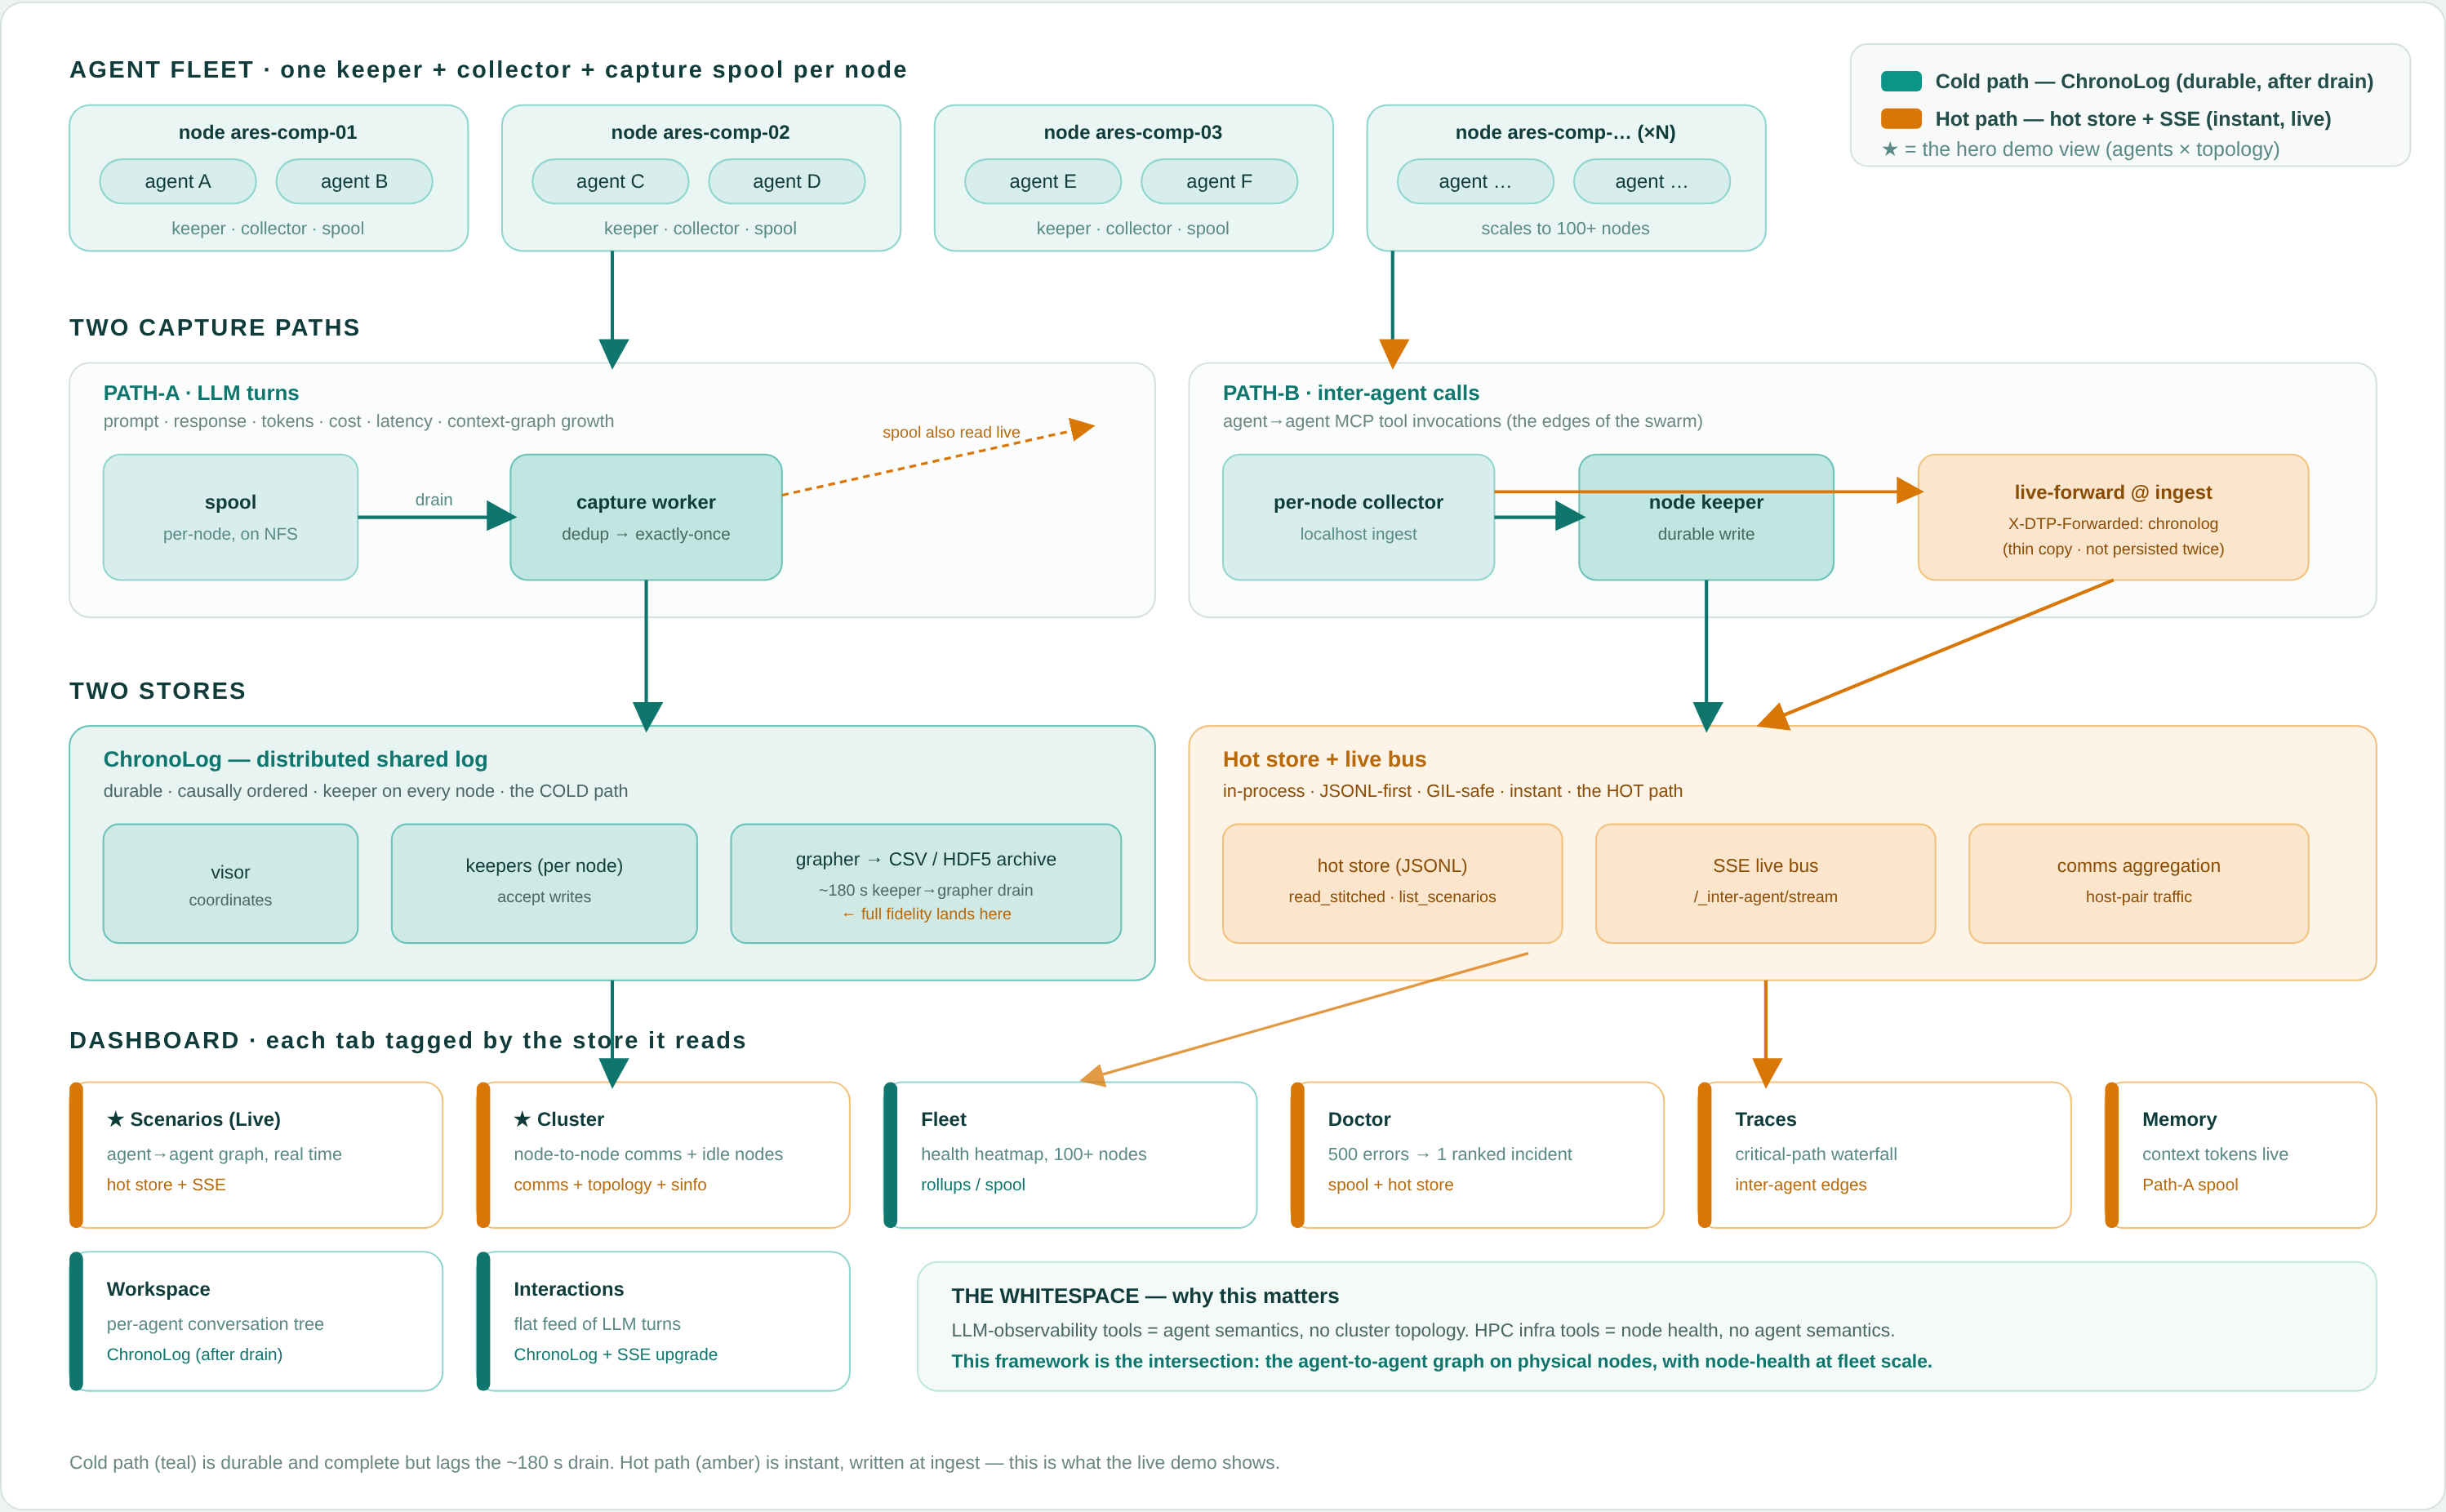
\includegraphics[width=\linewidth]{figures/dataflow}
  \caption{The two-path architecture. Path-A carries LLM turns through a
  node-local spool drained by a capture worker; Path-B carries inter-agent
  calls through a per-node collector. Both persist to ChronoLog through the
  node-local keeper; the dashboard reads ChronoLog (cold, full fidelity)
  and a local hot store (live).}
  \label{fig:dataflow}
\end{figure}

Every datum enters the system through one of two ingest paths
(Figure~\ref{fig:dataflow}), both terminating in ChronoLog via the keeper on
the producing node.

\textbf{Path-A} carries the intra-agent plane: LLM interactions (one record
per turn), context-graph deltas (one record per working-memory add or
eviction), and recovery events. Producers call a small capture library that
appends the record to a node-local, append-only \emph{spool}; a separate
\emph{capture worker} process periodically drains the spool into ChronoLog
stories.

\textbf{Path-B} carries the inter-agent plane: agent-to-agent MCP calls. Each
logical call is emitted as a \emph{pair} of events sharing a correlation
identifier: a \texttt{start} when the delegation is issued and a
\texttt{done} when it completes, the latter carrying status and latency. Agents
POST these events to a \emph{collector} daemon on their own node
(\texttt{localhost:5650}); the collector writes them to the node-local
ChronoLog keeper and simultaneously forwards a thin copy to the dashboard,
which feeds the live views (\S\ref{sec:design-read}).

The two paths differ deliberately. Path-A events are large (full prompts and
responses), produced at low rate (one per turn, i.e.\ per LLM call), and
consumed mostly after the fact, so a durable local buffer plus a batch
drain fits. Path-B events are small, structurally fixed, and latency-relevant (the live
scenario graph is drawn from them), and they define the cross-agent causal
structure; a daemon that stamps, persists, and immediately fans
them out is the better match. What the paths share is the destination and the discipline: node-local
append on the producing machine (R5), durable persistence in the log (R3),
and host attribution stamped at source (R1).

The dashboard itself is a \emph{pure reader}: a Flask application serving a
React single-page app that reconstructs every view from ChronoLog and the
hot store, and captures nothing on its own
(\S\ref{sec:design-isolation}).

\section{Mapping Agent Semantics onto the Log}
\label{sec:design-mapping}

ChronoLog organizes data as chronicle $\to$ story $\to$ event
(\S\ref{sec:bg-chronolog-model}). The mapping adopted here
(Table~\ref{tab:schema}) uses chronicles to partition by \emph{data kind}
and stories by \emph{entity}, so that every read pattern of
Chapter~\ref{chap:analytics} replays exactly one story:

\begin{table}[h]
\centering
\small
\begin{tabular}{@{}llll@{}}
\toprule
\textbf{Chronicle} & \textbf{Story} & \textbf{Holds} & \textbf{Path} \\
\midrule
\texttt{llm\_interactions} & \emph{session id} & LLM turns & A \\
\texttt{context\_graphs}   & \emph{session id} & working-memory deltas & A \\
\texttt{recovery\_events}  & \emph{session id} & recovery/backtrack events & A \\
\texttt{ia\_<scenario>}    & \texttt{edges}    & inter-agent \texttt{start}/\texttt{done} events & B \\
\texttt{metrics\_rollup}   & \texttt{minute}   & per-(host, minute) fleet buckets & rollup \\
\texttt{\_\_index\_\_}     & \texttt{scenarios} / \texttt{sessions} & listing index & both \\
\bottomrule
\end{tabular}
\caption{The chronicle/story schema: chronicles partition by data kind,
stories by entity. Session-scoped stories serve the conversation and
memory reads; the per-scenario edge story serves graph and trace reads;
the rollup and index stories are written by the capture side so that
readers never scan.}
\label{tab:schema}
\end{table}

\paragraph{Session identity.} The load-bearing convention is the session
identifier \texttt{role@scenario} (e.g.\ \texttt{writer@scenario-x}). It is
simultaneously the ChronoLog story name for all Path-A data of that agent,
the \texttt{from\_session}/\texttt{to\_session} endpoint on Path-B edges, and
the join key the dashboard uses when a clicked node in the scenario graph
opens that agent's conversation. Scoping the role by scenario keeps the
identifier globally unique across concurrent scenarios while leaving it
human-readable. Because the same string names the spool file, the
ChronoLog story, and the graph node, the identity round-trips through every
tier with no lookup table. This is R1's ``joinable planes'' made concrete:
the join is by construction, not by correlation heuristics.

\paragraph{Causal structure.} Cross-agent causality is carried by two
explicit fields on Path-B events. The \texttt{correlation\_id} stitches the
\texttt{start}/\texttt{done} pair of one call into a single edge; the
optional \texttt{parent\_correlation\_id} records the call being
\emph{serviced} when a new call was issued, giving the tracer exact call
trees. When instrumentation does not propagate the parent, the tracer falls
back to inference from session identity and time nesting
(\S\ref{sec:analytics-tracing}), the Mystery-Machine position on the
spectrum of \S\ref{sec:bg-tracing-lineage}, with explicit propagation as the
Dapper position when available. Within a session, Path-A records carry a
monotonic per-stream \texttt{sequence\_id}, which orders turns without
reference to wall clocks.

\paragraph{Listing without enumeration.} One practical gap in the substrate
is the absence of a chronicle-enumeration operation in the client binding:
there is no way to ask ``which scenarios exist?'' without knowing their
names. The design routes around it with an \texttt{\_\_index\_\_} chronicle:
every component that first sees a new scenario or session appends a one-line
event (\texttt{\{"v": <name>\}}) to a well-known index story, and listing
becomes a replay of that story, deduplicated in first-seen order. The index
is append-only and idempotent to re-add, so it needs no coordination among
the writers. The pattern is a small instance of the log-as-substrate principle: when a
query is missing, materialize it as another log.

\section{Write Path and Delivery Semantics}
\label{sec:design-write}

The write path is engineered backwards from R5 (never perturb the agent) and
R3 (never lose, never duplicate).

\paragraph{The spool as write-ahead buffer.} A Path-A producer's fast path is
an append of one JSON line to a per-\((\text{session}, \text{kind})\) spool
file, opened with \texttt{O\_APPEND} so that concurrent writers interleave
atomically at line granularity. No network, no lock, no dependency on any
downstream component being alive: if ChronoLog, the capture worker, or the
dashboard is down, agents keep running and the spool absorbs the backlog.
The capture library injects and guarantees exactly three fields:
\texttt{session\_id}, a monotonic \texttt{sequence\_id} (seeded from the
maximum found on disk, so monotonicity survives producer restarts), and a
\texttt{timestamp}. It treats the rest of the record as an opaque
producer contract.

\paragraph{Effectively exactly-once ingest.} The capture worker drains the
spool into ChronoLog on a polling interval. Transport is at-least-once by
construction (after a crash the worker re-reads spool files it may have
partially drained), so ingest must deduplicate. The worker keeps a
\emph{high-water mark} per \((\text{session}, \text{kind})\) stream: the
largest \texttt{sequence\_id} already written to ChronoLog. Only records
above the mark are appended. The critical property is where that state
lives: on startup the worker \emph{rebuilds the marks from ChronoLog
itself}, replaying each session's stories to find the highest sequence
present. The log is thus the single source of truth for what has been
ingested, and the worker carries no durable state of its own. No worker
crash, restart, or migration to another node can cause loss (the spool
retains everything) or duplication (the rebuilt marks skip everything
already present). Records without a natural sequence (recovery events) carry
a unique blob identifier and are deduplicated by set membership, seeded the
same way. The arrangement is the textbook recipe of \S\ref{sec:bg-delivery}
(at-least-once transport plus idempotent, monotonic ingest), instantiated
with the log as its own ledger.

\paragraph{Path-B: persist once per backend.} The collector gives Path-B
events the same guarantees with one extra subtlety. Every event travels to
\emph{two} places: the node-local keeper (durable) and the dashboard (for
the live bus). Naively this double-writes. The design makes the forward
explicit: when, and only when, the collector has successfully written an
event to ChronoLog, it sets a header (\texttt{X-DTP-Forwarded: chronolog})
on the forwarded copy. The dashboard honors the header by preserving the
collector-stamped identifiers verbatim and skipping its own ChronoLog write,
storing only the hot copy. If the keeper write failed, the collector
forwards \emph{without} the header and the dashboard persists the event
through its own backend; the placement is degraded, but the event is
not lost. The net
contract: each event is persisted exactly once per backend, and the
identifiers (\texttt{event\_id}, timestamps) are identical in both copies,
so the live view and the durable view never disagree about identity.

\paragraph{Graceful degradation.} One more fallback closes the path: an
agent's \texttt{emit()} tries the node-local collector first and falls back
to POSTing directly to the dashboard's ingest endpoint if the collector is
down. The fallback sends no forwarded header, so the dashboard persists
normally. An agent therefore observes at most a failed local HTTP call
before falling back: never a lost edge, and never back-pressure from the
log (R5).

\section{The Read Problem: Hot and Cold Paths}
\label{sec:design-read}

Writing to an ingest-optimized log is easy; reading it live is the hard
part. As established in \S\ref{sec:bg-chronolog-design}, freshly appended
events sit inside the keeper$\to$grapher acceptance window
(20--30\,s measured end-to-end in the deployments used here) before they
are readable from the archive. Worse, a replay the player cannot
answer does not return stale data but \emph{blocks} for the client's
${\sim}180$\,s query timeout, in a Python client that holds the GIL
throughout. A dashboard
that naively replayed stories on request would freeze for minutes precisely
while the fleet is live, a direct violation of R2.

The design response is a lambda-style split (\S\ref{sec:bg-log}) with the
acceptance window as the boundary:

\paragraph{The cold path} is ChronoLog itself: complete, durable, ordered,
and authoritative, but late. Full-fidelity views (a session's complete
conversation, post-hoc analysis) read it, either by live replay once a story
has drained or from the grapher's archive files. Reads that risk touching
un-drained state are avoided structurally: the listing index of
\S\ref{sec:design-mapping} is read \emph{archive-first}, because a live
replay against a never-written index story blocks indefinitely
(\S\ref{sec:design-isolation}). The evaluation later hardened this rule
into a deployment mode: after live replay proved unreliable end-to-end
on the cluster, archive-first reading was generalized from
the listing index to \emph{every} replay the serving processes issue,
bounding staleness at the drain window
(\S\ref{sec:eval-freshness}, \S\ref{sec:eval-limitations}).

\paragraph{The hot path} serves R2 and is populated \emph{at the moment of
ingest}, before ChronoLog acceptance. It has two elements. First, a
\emph{hot store}: the ingest endpoint appends every Path-B event to a local
JSONL file per scenario, and all live read APIs (the scenario graph, the
node-communication view, fleet aggregation, the tracer) read this store,
an instant, append-only local read that can never block on the log. Second,
a \emph{live bus}: an in-process publish/subscribe fan-out that pushes each
newly ingested event to server-sent-event subscribers, so the browser
renders edges as they happen rather than polling. Path-A has the analogous
arrangement: the Health view and the per-agent memory panels read the
capture spool directly (the spool doubling as Path-A's hot store)
while ChronoLog remains the durable copy.

\paragraph{The late-join protocol.} A client that opens a live stream
mid-run needs history plus continuity without gaps or duplicates. The bus
protocol delivers the stored backlog first, then live frames, and the
subscription is registered \emph{before} the backlog is read, so an
event ingested during the handoff appears in both, and the client
deduplicates by event identifier. Delivery to subscribers is intentionally
weaker than delivery to storage: per-subscriber queues are bounded and drop
oldest under pressure, and a publish never blocks or raises into the ingest
path. By the time an event reaches the bus it is already durable, so the
live stream is a best-effort projection of a reliable log, not a second
reliability domain (R5).

\paragraph{Consistency model.} Each view advertises, in effect, one of two
freshness classes: hot views are eventually consistent with the log but
fresh to within the ingest latency (measured in
Chapter~\ref{chap:evaluation}); cold views are complete and ordered but
stale up to the acceptance window. Because both are projections of the same
event stream with identical identifiers
(\S\ref{sec:design-write}), the classes converge: after the drain, a hot
view's content is a prefix-complete subset of the cold view's, and the
operator can always escalate from ``live picture now'' to ``authoritative
record later'' without changing tools.

\section{Process and Failure Isolation}
\label{sec:design-isolation}

The deployment decomposes into single-responsibility processes per node
(agents, collector, capture worker), plus one dashboard for the
allocation. Three isolation rules, each learned from a concrete failure on
live clusters, govern the decomposition.

\paragraph{The dashboard is a pure reader.} An early configuration ran the
capture worker as a thread inside the dashboard process. On startup the
worker warms its high-water marks by replaying sessions
(\S\ref{sec:design-write}); on a cluster where a story sat inside the
acceptance window, that replay blocked while holding the GIL, and the Flask
server never finished binding its port. The lesson generalizes: a process
that must always answer (the dashboard) may never share an interpreter with
a component that may legitimately block on remote state (the capture
worker). They now run as separate processes, and the rule extends to reads:
no request handler ever issues a replay that could touch un-drained state.

\paragraph{Never block on state that may not exist.} A fresh cluster
exhibits a boundary case. Replaying an index story that has \emph{never
been written} blocks indefinitely: there is no data to drain, and none
will ever arrive. Listing reads are therefore archive-first (the archive's
absence is detectable instantly, while a live replay's futility is not),
with live replay behind an explicit opt-in; and a brand-new deployment
seeds the index with a one-shot append-only sync pass, sidestepping the
blocking warm-up entirely.

\paragraph{Normalize identity at the edge.} Host names arrive from multiple
authorities (reverse DNS reports \texttt{ares-comp-3}, SLURM reports
\texttt{ares-comp-03}), and any view that joins on host names (fleet
health, the cluster graph, allocation membership) silently drops nodes if
the two spellings coexist. All host names are therefore canonicalized (digit
padding stripped) at every boundary where they enter a data structure.
Identity normalization, like time, belongs at the edge of the system, not
in each consumer.

Failure containment follows from the decomposition: an agent crash loses
nothing already spooled or emitted; a collector crash falls agents back to
direct dashboard ingest; a capture-worker crash pauses draining while the
spool absorbs; a dashboard crash affects only observation (capture
continues); and a ChronoLog outage degrades the system to hot-store-only
operation, with the spool and collector queues replaying into the log when
it returns.

\section{Extensibility: Adapters and Capabilities}
\label{sec:design-adapters}

Every dashboard view is declared as a \emph{capability} (conversations,
scenarios, diagnostics, fleet, tracing, \dots) served by a \emph{source
adapter}, an interface discovered at runtime through a Python
entry-point group. The shipped ChronoLog adapter serves all capabilities;
at startup the application discovers active adapters, mounts only the API
blueprints some adapter can serve, and advertises the active set to the
frontend, which renders only those tabs. The seam exists for third parties:
a deployment with a different substrate implements the adapter interface
and gains the dashboard unchanged. The same seam is what
makes the offline demo mode (local stores, no cluster) a configuration
rather than a fork. This chapter's design is thereby separable: the capture
paths, delivery semantics, and hot/cold split of
\S\S\ref{sec:design-write}--\ref{sec:design-read} are ChronoLog-specific
engineering; the analytics of Chapter~\ref{chap:analytics} depend only on
the capability interface.

\chapter{Fleet-Scale Analytics on the Log}
\label{chap:analytics}

Chapter~\ref{chap:design} produced a substrate: every observable event of
the fleet, durably ordered, attributed to node and agent, readable hot or
cold. This chapter presents the analyses that turn that substrate into
answers to the operator questions of \S\ref{sec:problem-scenario}. Each
section follows the same shape: the question, the algorithm, and the
argument for why it stays cheap at fleet scale.

\section{Live Topology Coupling: Scenario Graph and Cluster Graph}
\label{sec:analytics-topology}

The first question (Q1) is situational awareness: what is the swarm doing,
right now, and where. The system answers it with two live graphs, built
deliberately as \emph{two projections of the same event stream}.

The \emph{scenario graph} projects Path-B edges onto agent identity: nodes
are sessions (\texttt{role@scenario}), edges are stitched calls labeled
with tool, status, and latency, built incrementally in the browser from the
live bus: backlog first, then per-event frames
(\S\ref{sec:design-read}). LLM-observability tools already offer this view
(\S\ref{sec:bg-sota-llm}); here it is rendered live. The \emph{cluster graph} projects
the very same edges onto physical topology: hosts as nodes, aggregated
host-pair traffic as edges (counts, error counts, active agents per host),
computed by folding the hot store. Because every edge carries
\texttt{from\_host} and \texttt{to\_host} stamped at capture (R1), the
projection is a group-by, not an inference.

The coupling is completed by the scheduler's view of the machine: the
dashboard queries SLURM (\texttt{sinfo}) for the allocation and the
cluster's total/idle/busy/down states, draws idle-but-available nodes
alongside the active deployment, and uses only real node names throughout.
A node with no events is drawn grey, not omitted; at fleet scale,
silence is a signal (R4). Clicking through connects the layers: an agent
node opens that agent's conversation (the \texttt{role@scenario} join of
\S\ref{sec:design-mapping}); a host cell pivots to the per-node view. This
two-projection design (same events, agent layer and machine layer) is
the direct answer to the gap of \S\ref{sec:bg-sota-gap}.

\section{ChronoDoctor: Detection, Clustering, and Diagnosis}
\label{sec:analytics-doctor}

The second question (Q2) is not ``show me the errors'' but ``tell me what
is wrong'': at fleet scale, a per-event error feed is least readable
when it matters most. ChronoDoctor is a five-stage pipeline
(\emph{gather} $\to$ \emph{detect} $\to$ \emph{cluster} $\to$
\emph{diagnose} $\to$ \emph{remember}) that turns raw events into a
ranked list of explained incidents.

\paragraph{Gather and detect.} Gathering is the only I/O: interactions and
recoveries from the Path-A spool (hot, GIL-safe), stitched edges from the
Path-B hot store, with explicit bounds on sessions and scenarios scanned.
Detection is a set of pure, unit-tested functions over the gathered lists,
each emitting typed \emph{signals}: HTTP 4xx/5xx and explicit errors on
turns (429 classified separately as rate-limiting); latency outliers,
flagged relative to the \emph{per-model} median (an absolute threshold
would misclassify a slow model as an incident); retry storms (the same
prompt re-issued repeatedly within a session); failed inter-agent calls;
\emph{orphan calls} (a \texttt{start} with no \texttt{done}, the
signature of a hung or dropped delegation); slow edges relative to the
per-tool median; and recovery events. Orphan calls are always ranked
critical: the delegating agent is silently stalled, and no per-edge view
shows anything wrong.
Detection is a single pass: $O(n)$ in gathered events, with per-group
medians over small per-model and per-tool groups.

\paragraph{Clustering.} The insight that makes the view scale is that
fleet-wide failures are \emph{textually self-similar}. Each signal's
message is normalized, with identifiers, hex runs, and digit strings replaced
by placeholders (\texttt{peer ares-comp-12 timed out after 30001ms}
$\to$ \texttt{peer ares-comp-<n> timed out after <n>ms}), and the pair
(kind, normalized message) is hashed into a \emph{signature}, the
clustering key. Five hundred identical timeouts across the fleet collapse
into one incident with a count of 500; hosts, sessions, tools, models, and
scenarios are aggregated \emph{inside} the incident as its blast radius,
deliberately excluded from the key so that a fleet-wide failure stays one
card while its distribution stays visible. Severity escalates with count,
and incidents rank by (severity, count, hosts affected), worst first.

\paragraph{Diagnosis.} Each incident gets a diagnosis (root cause,
remediation, blast radius, confidence) from a deterministic,
first-match-wins rule engine keyed on signal kind and sample text: orphan
calls map to hung-peer causes, 429s to rate limiting, transport-layer
markers to network-fabric issues, token-overflow patterns to context
exhaustion, and so on, each with a calibrated confidence; a conservative
fallback catches the rest. The engine costs nothing per scan (R6). An
LLM-backed diagnoser can be enabled explicitly, and any failure of it falls
back to the heuristic: the deterministic path is the contract, the LLM
an enhancement.

\paragraph{Memory.} The final stage answers Q5. Every scan appends one line
per incident to a Markdown incident memory; when the recent section
exceeds a threshold, the oldest lines fold into a digest with running
counts; the file is \emph{self-compacting}, so it stays small across
arbitrarily many runs while retaining per-signature totals. On each scan,
current incidents are matched against remembered signatures, and a repeat
offender is badged \texttt{recurring $\times N$}. The memory is a plain
human-readable file: the operator can read, annotate, or delete it, and it
survives restarts by construction.

\section{Fleet Health at Scale}
\label{sec:analytics-fleet}

The fourth question (Q4) is population-level: which node is unlike the
others. The node-link rendering of \S\ref{sec:analytics-topology} answers
it only up to a dozen nodes; past that, it is spaghetti. The fleet view
therefore changes representation (a heatmap grid, one cell per node,
colored by health, worst first) and, more fundamentally, changes the
\emph{read complexity}.

Computing node health from raw events is $O(\text{events})$ per refresh,
untenable as history grows. The system instead maintains
\emph{rollups}: for each (host, minute) pair, a bucket aggregating that
minute's activity (event and error counts, latency sum/count/p95/max,
token and cost totals, distinct agents). An emitter recomputes and appends
full bucket snapshots to a dedicated rollup story; because each append is a
complete snapshot of its cell, the reader keeps the last value seen per key
and re-emission never double-counts: idempotence by
last-writer-wins, the same discipline as \S\ref{sec:design-write}. A
health query then folds only the buckets in the requested window:
$O(\text{nodes} \times \text{buckets})$, independent of event volume (R4).
Per-node health folds by explicit rules: sums for counts, a ratio for
error rate, and the \emph{maximum} of per-minute p95s as the
window's p95 estimate (an upper-biased estimate that avoids retaining raw
samples). Thresholds then classify each node ok/warn/critical. Nodes in
the allocation that produced nothing are injected as empty rows, and every
row is tagged with its live SLURM state, so the grid always shows the
whole population. The emitter is optional. Absent rollups, the API falls
back to folding raw events on demand, which is correct at small scale and
keeps the tab from ever being empty.

\section{Cross-Host Critical-Path Tracing}
\label{sec:analytics-tracing}

The third question (Q3), why this scenario is slow, is the classical
tracing question of \S\ref{sec:bg-tracing}, posed across hosts. The tracer
reconstructs call trees from stitched Path-B edges in two steps.

\paragraph{Tree reconstruction.} Each stitched edge is a span: an interval
on the timeline from \texttt{start} to \texttt{done}, with endpoints,
tool, status, and latency. Parentage is resolved by a two-tier rule
mirroring \S\ref{sec:design-mapping}: if a span carries an explicit
\texttt{parent\_correlation\_id}, that is its parent, the
Dapper-style ground truth. Otherwise the parent is \emph{inferred}: the
span whose callee session matches this span's caller session and whose
interval encloses this span's (the tightest such enclosure winning),
on the Mystery-Machine premise that a delegation issued by agent $B$ while
$B$ was servicing a call must be causally nested within it. Spans with no
parent are roots; each root yields one trace, with depth assigned by tree
walk.

\paragraph{Critical path and bottleneck.} Within a trace, end-to-end
latency is attributed by the analysis of \S\ref{sec:bg-critpath}: the
critical path is walked from the root by descending into the slowest
child at each level, and each hop on the path is charged its
\emph{self-time} (its latency minus its slowest child's), so that
time spent waiting on a child is charged to the child, not double-counted
in the parent. The hop with maximal self-time is named the
\emph{bottleneck}, with its hosts and tool: not ``the scenario is slow''
but ``the \texttt{writer}$\to$\texttt{reviewer} hop on
\texttt{ares-comp-07}, 4.2\,s of self-time.'' Because hosts ride on every
span, the pivot to Q4 is immediate: if the bottleneck's node also glows in
the fleet heatmap, the cross-layer diagnosis (fleet symptom, physical
cause) completes in two clicks. Chapter~\ref{chap:evaluation} follows
exactly this pivot as a case study. The waterfall
rendering shows the trace with depth indentation and the critical path
highlighted; reconstruction is $O(s^2)$ in the spans of a scenario in the
inference case ($s$ small, tens of calls) and $O(s)$ with explicit
parents.

\section{The Operator Surface: Five Views over One Log}
\label{sec:analytics-surface}

Everything in this chapter and the last is, from the operator's chair,
five tabs in one dashboard. Each view is a projection of the same
captured event stream (none holds private state that is not
reconstructible from the log), and each exists to answer one of the
operator questions of \S\ref{sec:problem-scenario}. This section walks
the surface as an operator sees it; Figures~\ref{fig:ui-scenarios}
through~\ref{fig:ui-traces} are captures of the deployed system.

\paragraph{Scenarios: who is talking to whom
(Fig.~\ref{fig:ui-scenarios}).} The dashboard opens here. One scenario is
selected from the left rail, its agents drawn as peers grouped into host
containers, every inter-agent call an animated edge (color-coded by
status, errors in red). The header carries the scenario's live totals
(hosts, agents, messages, errors) and a \emph{Live/Full} toggle:
\emph{Live} renders from the hot store and SSE bus as events arrive;
\emph{Full} re-reads the drained archive for complete fidelity,
including a replay scrubber that re-animates history at chosen speed.
Clicking any agent, host box, or edge opens its detail panel; from an
agent the operator can pivot into its full conversation (the turns,
token counts, and costs behind the node), which is the Q1 join of
capture to conversation, exercised end-to-end by the functional
harness of \S\ref{sec:eval-functional}.

\begin{figure}[p]
  \centering
  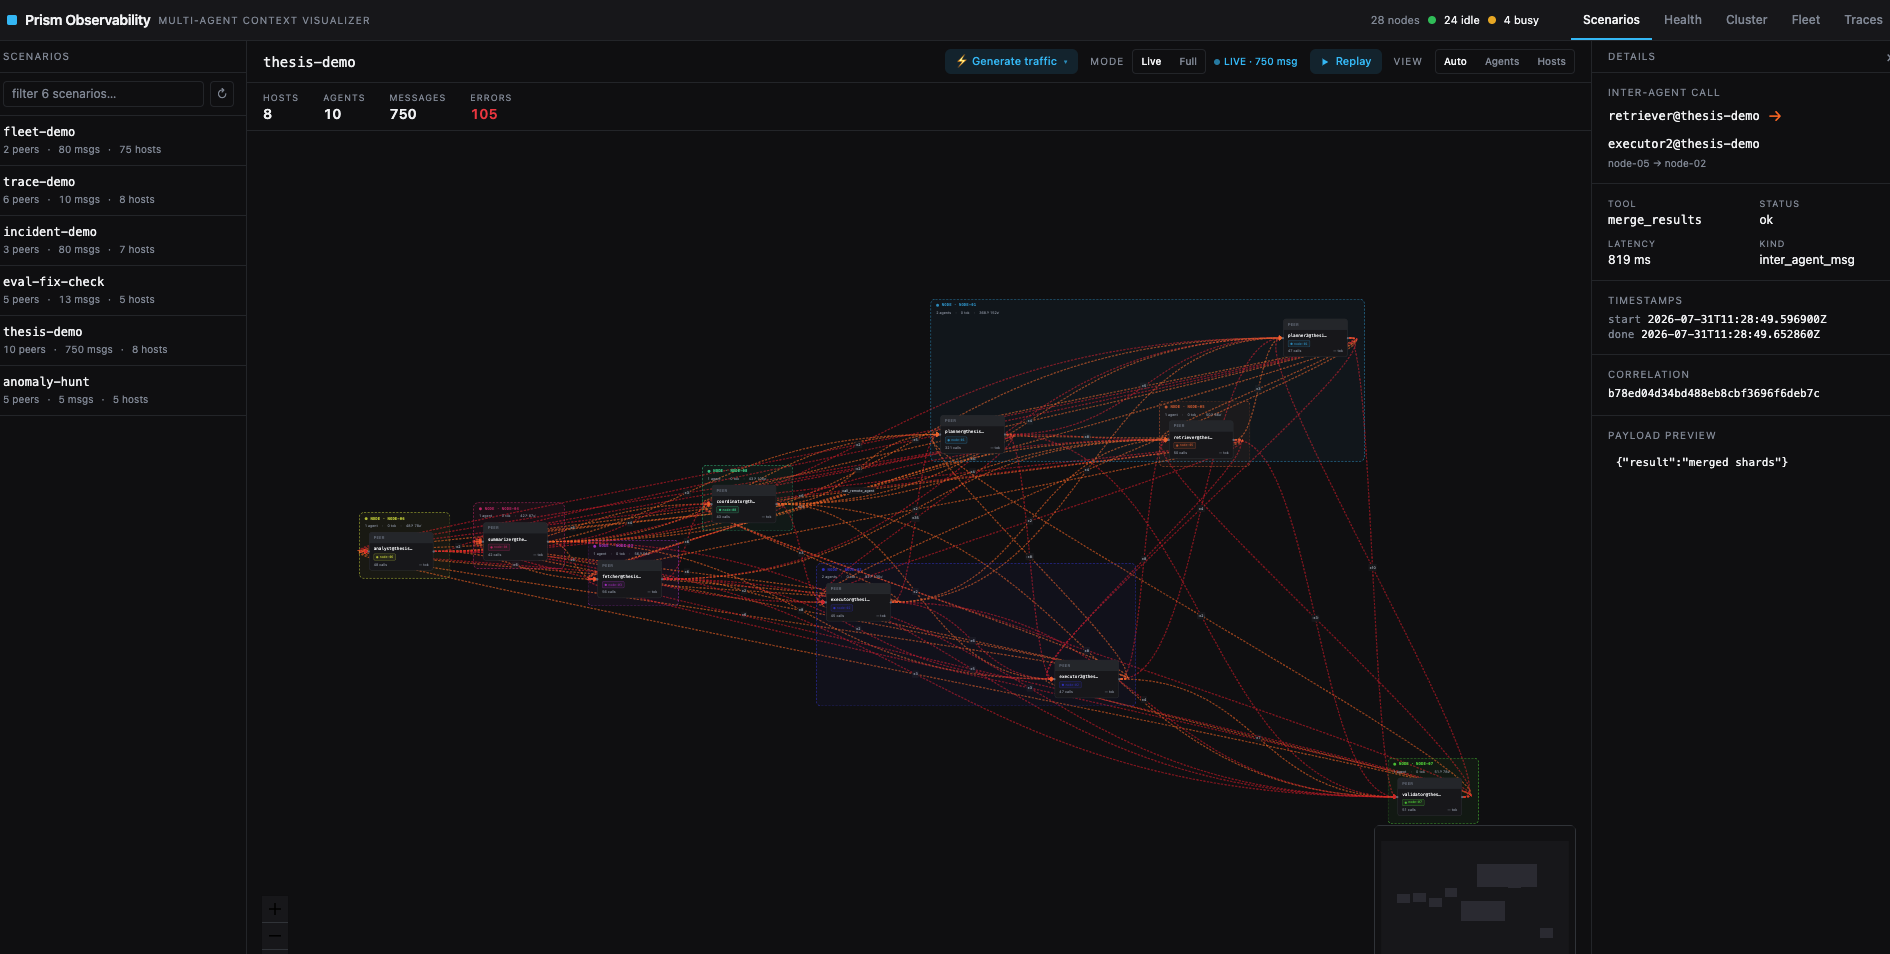
\includegraphics[width=\linewidth]{figures/ui-scenarios}
  \caption{The Scenarios view, live: 10 agents across 8 host groups,
  every inter-agent call an edge (errors red), with live message and
  error counters. Clicking a node opens the agent's conversation,
  the capture-to-conversation join of R1.}
  \label{fig:ui-scenarios}
\end{figure}

\paragraph{Health: what is wrong, and why
(Fig.~\ref{fig:ui-health}).} The ChronoDoctor surface. The center
column is the live LLM-call feed (every turn as it happens, filterable
to errors or a provider); the left rail is the ranked incident list a
scan produces: one card per clustered incident, ordered by severity,
with occurrence counts and \emph{recurring} badges read back from the
incident memory. Selecting an incident opens its diagnosis card:
\emph{why this is happening} and \emph{how to fix it} in prose, the
blast radius (occurrences, hosts, agents, scenarios), the heuristic's
stated confidence, and the raw evidence samples that justify it.
The compression argument of \S\ref{sec:analytics-doctor} is legible in
the ratio: thousands of raw signals arrive as a dozen ranked cards, each
carrying its own justification.

\begin{figure}[p]
  \centering
  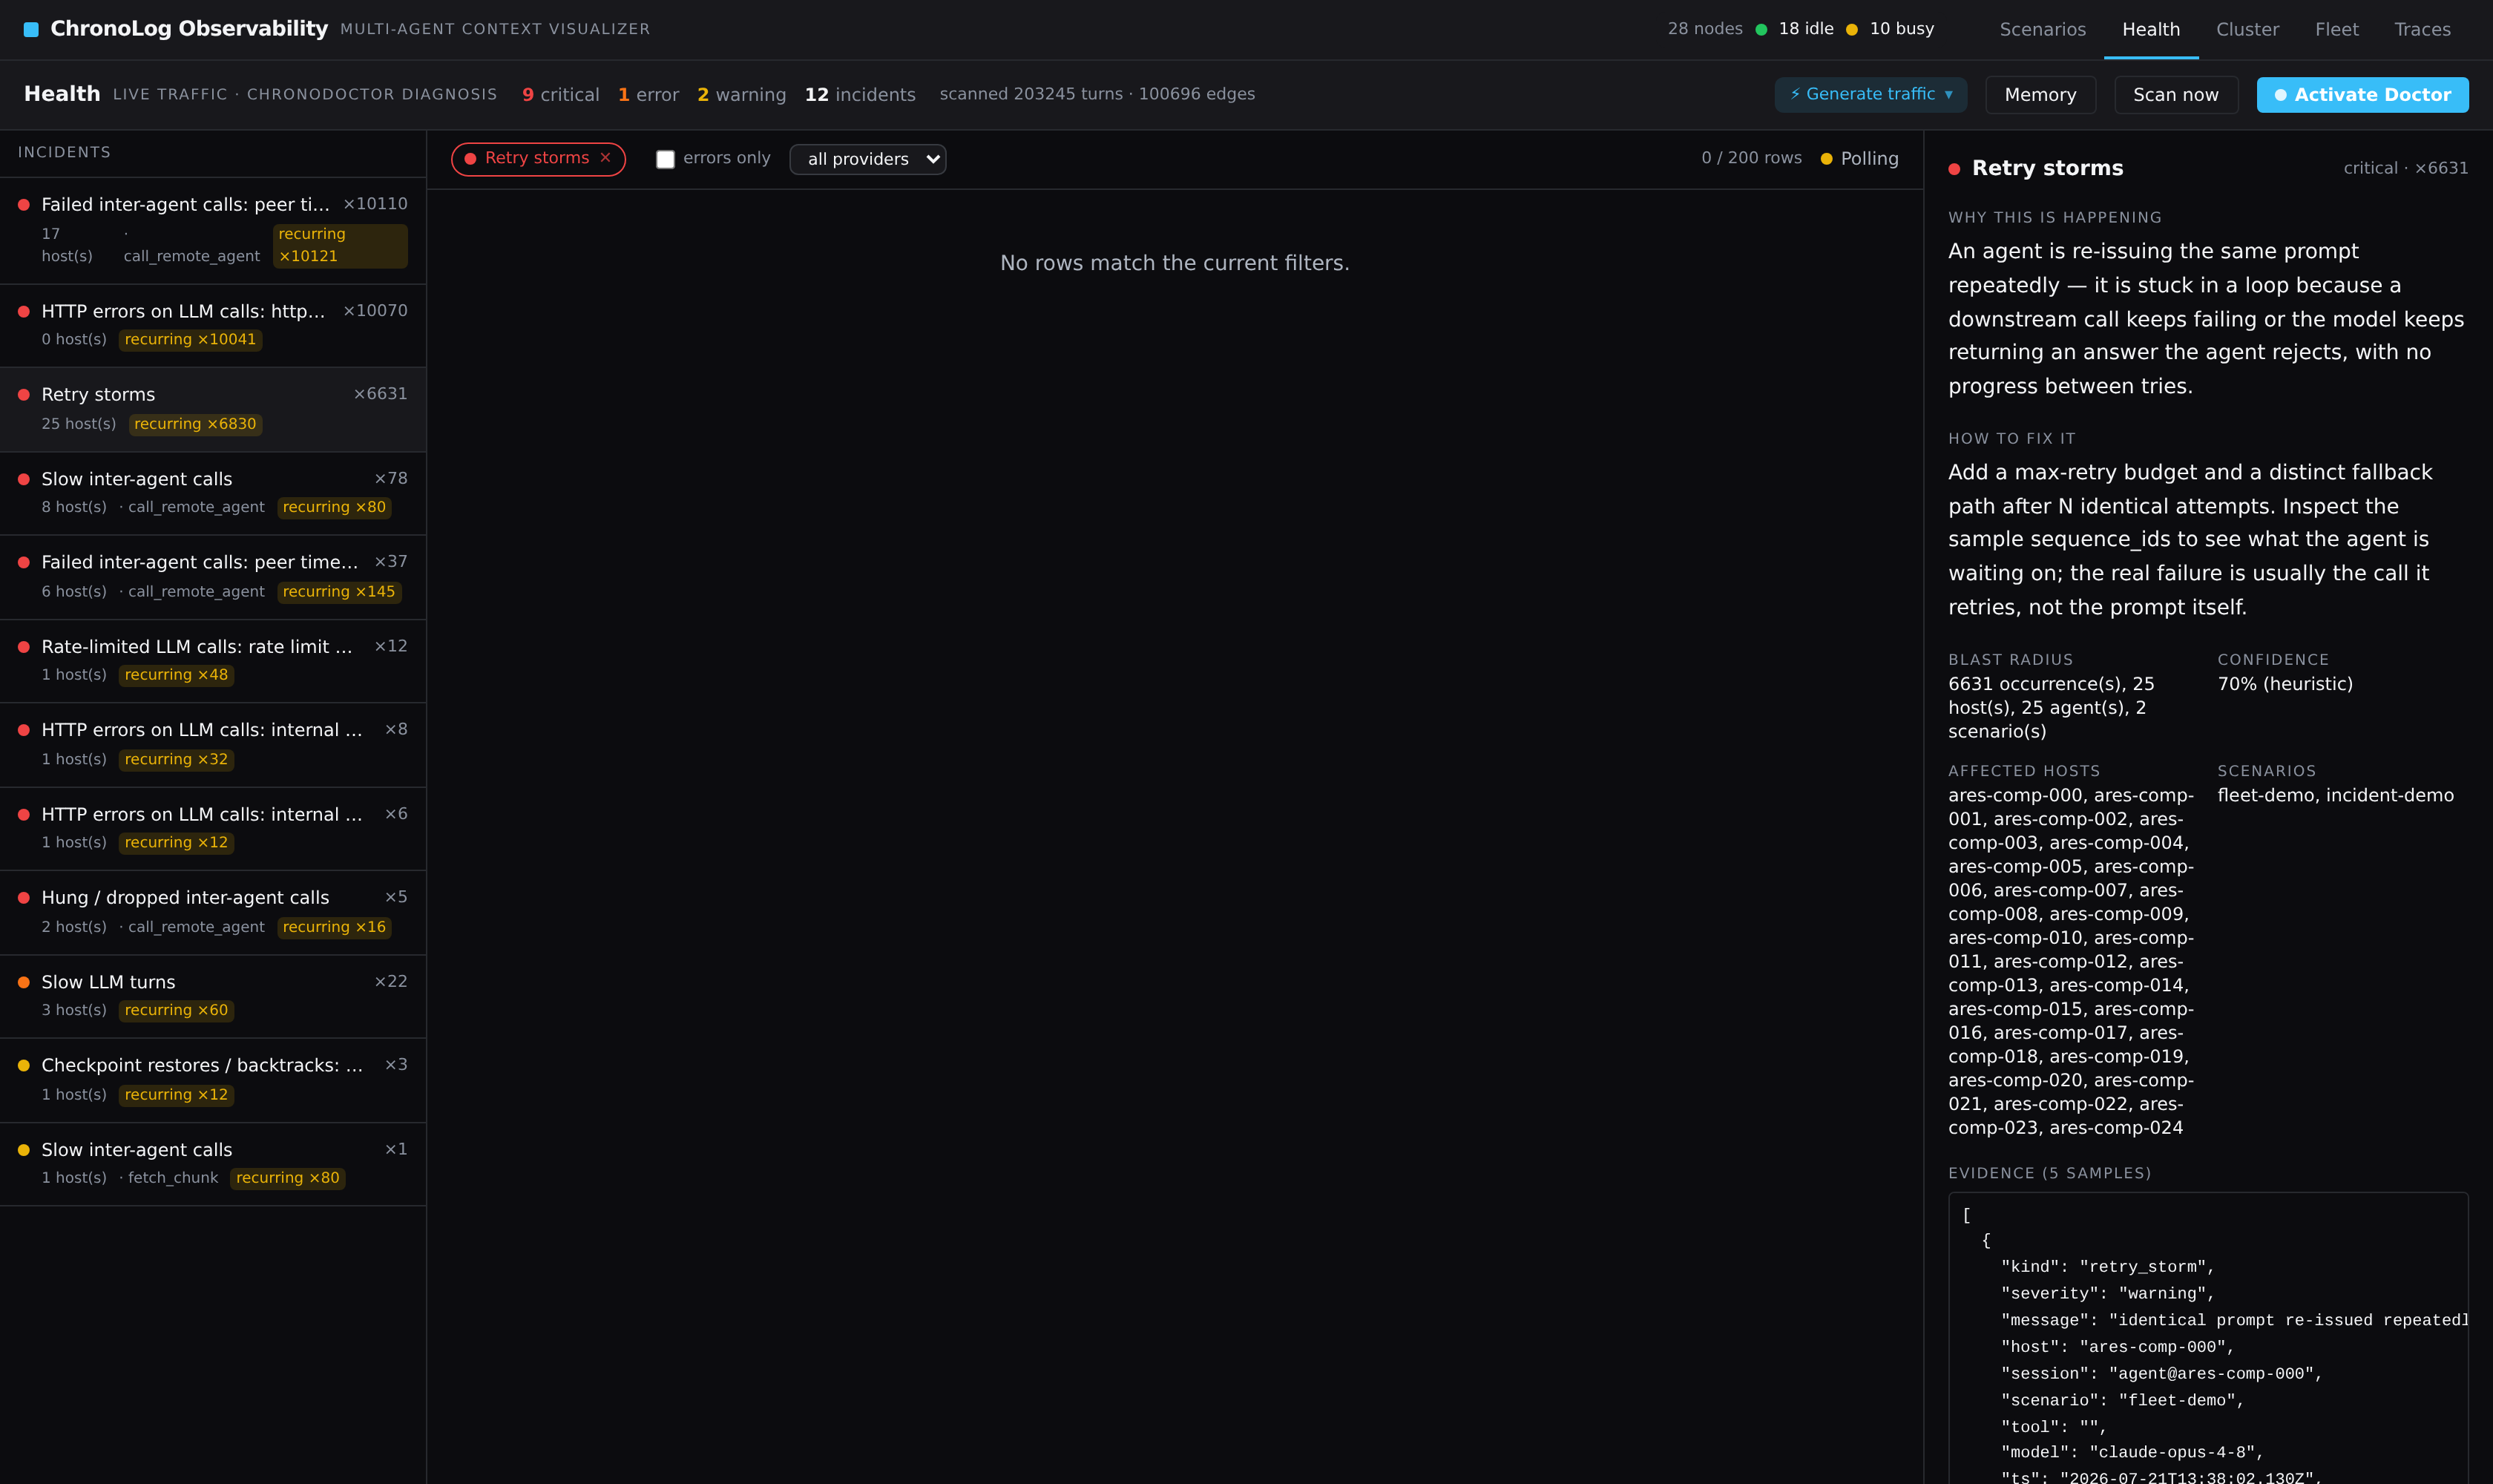
\includegraphics[width=\linewidth]{figures/ui-health}
  \caption{The Health view after a Doctor scan over a large demo
  corpus: 12 ranked incidents from ${\sim}200$\,k scanned turns (left),
  and the selected incident's diagnosis card (right) carrying root cause,
  remediation, blast radius, confidence, and evidence samples.
  \emph{Recurring} badges are read from the cross-run incident memory.}
  \label{fig:ui-health}
\end{figure}

\paragraph{Cluster: agent semantics on physical topology
(Fig.~\ref{fig:ui-cluster}).} This view puts the substrate itself on
screen: the ChronoLog
deployment drawn on the allocation's nodes (visor, one keeper
card per node with the chronicles and stories it holds, grapher and
player placement), overlaid with the cluster graph of
\S\ref{sec:analytics-topology} so that
agent traffic is visible \emph{on} the machines that carry it, next to
the SLURM capacity badge (idle/busy/down). R7 reads directly off the
picture: the same physical node hosts both an agent's runtime and
the keeper that captures it, and the operator sees both roles at once.

\begin{figure}[p]
  \centering
  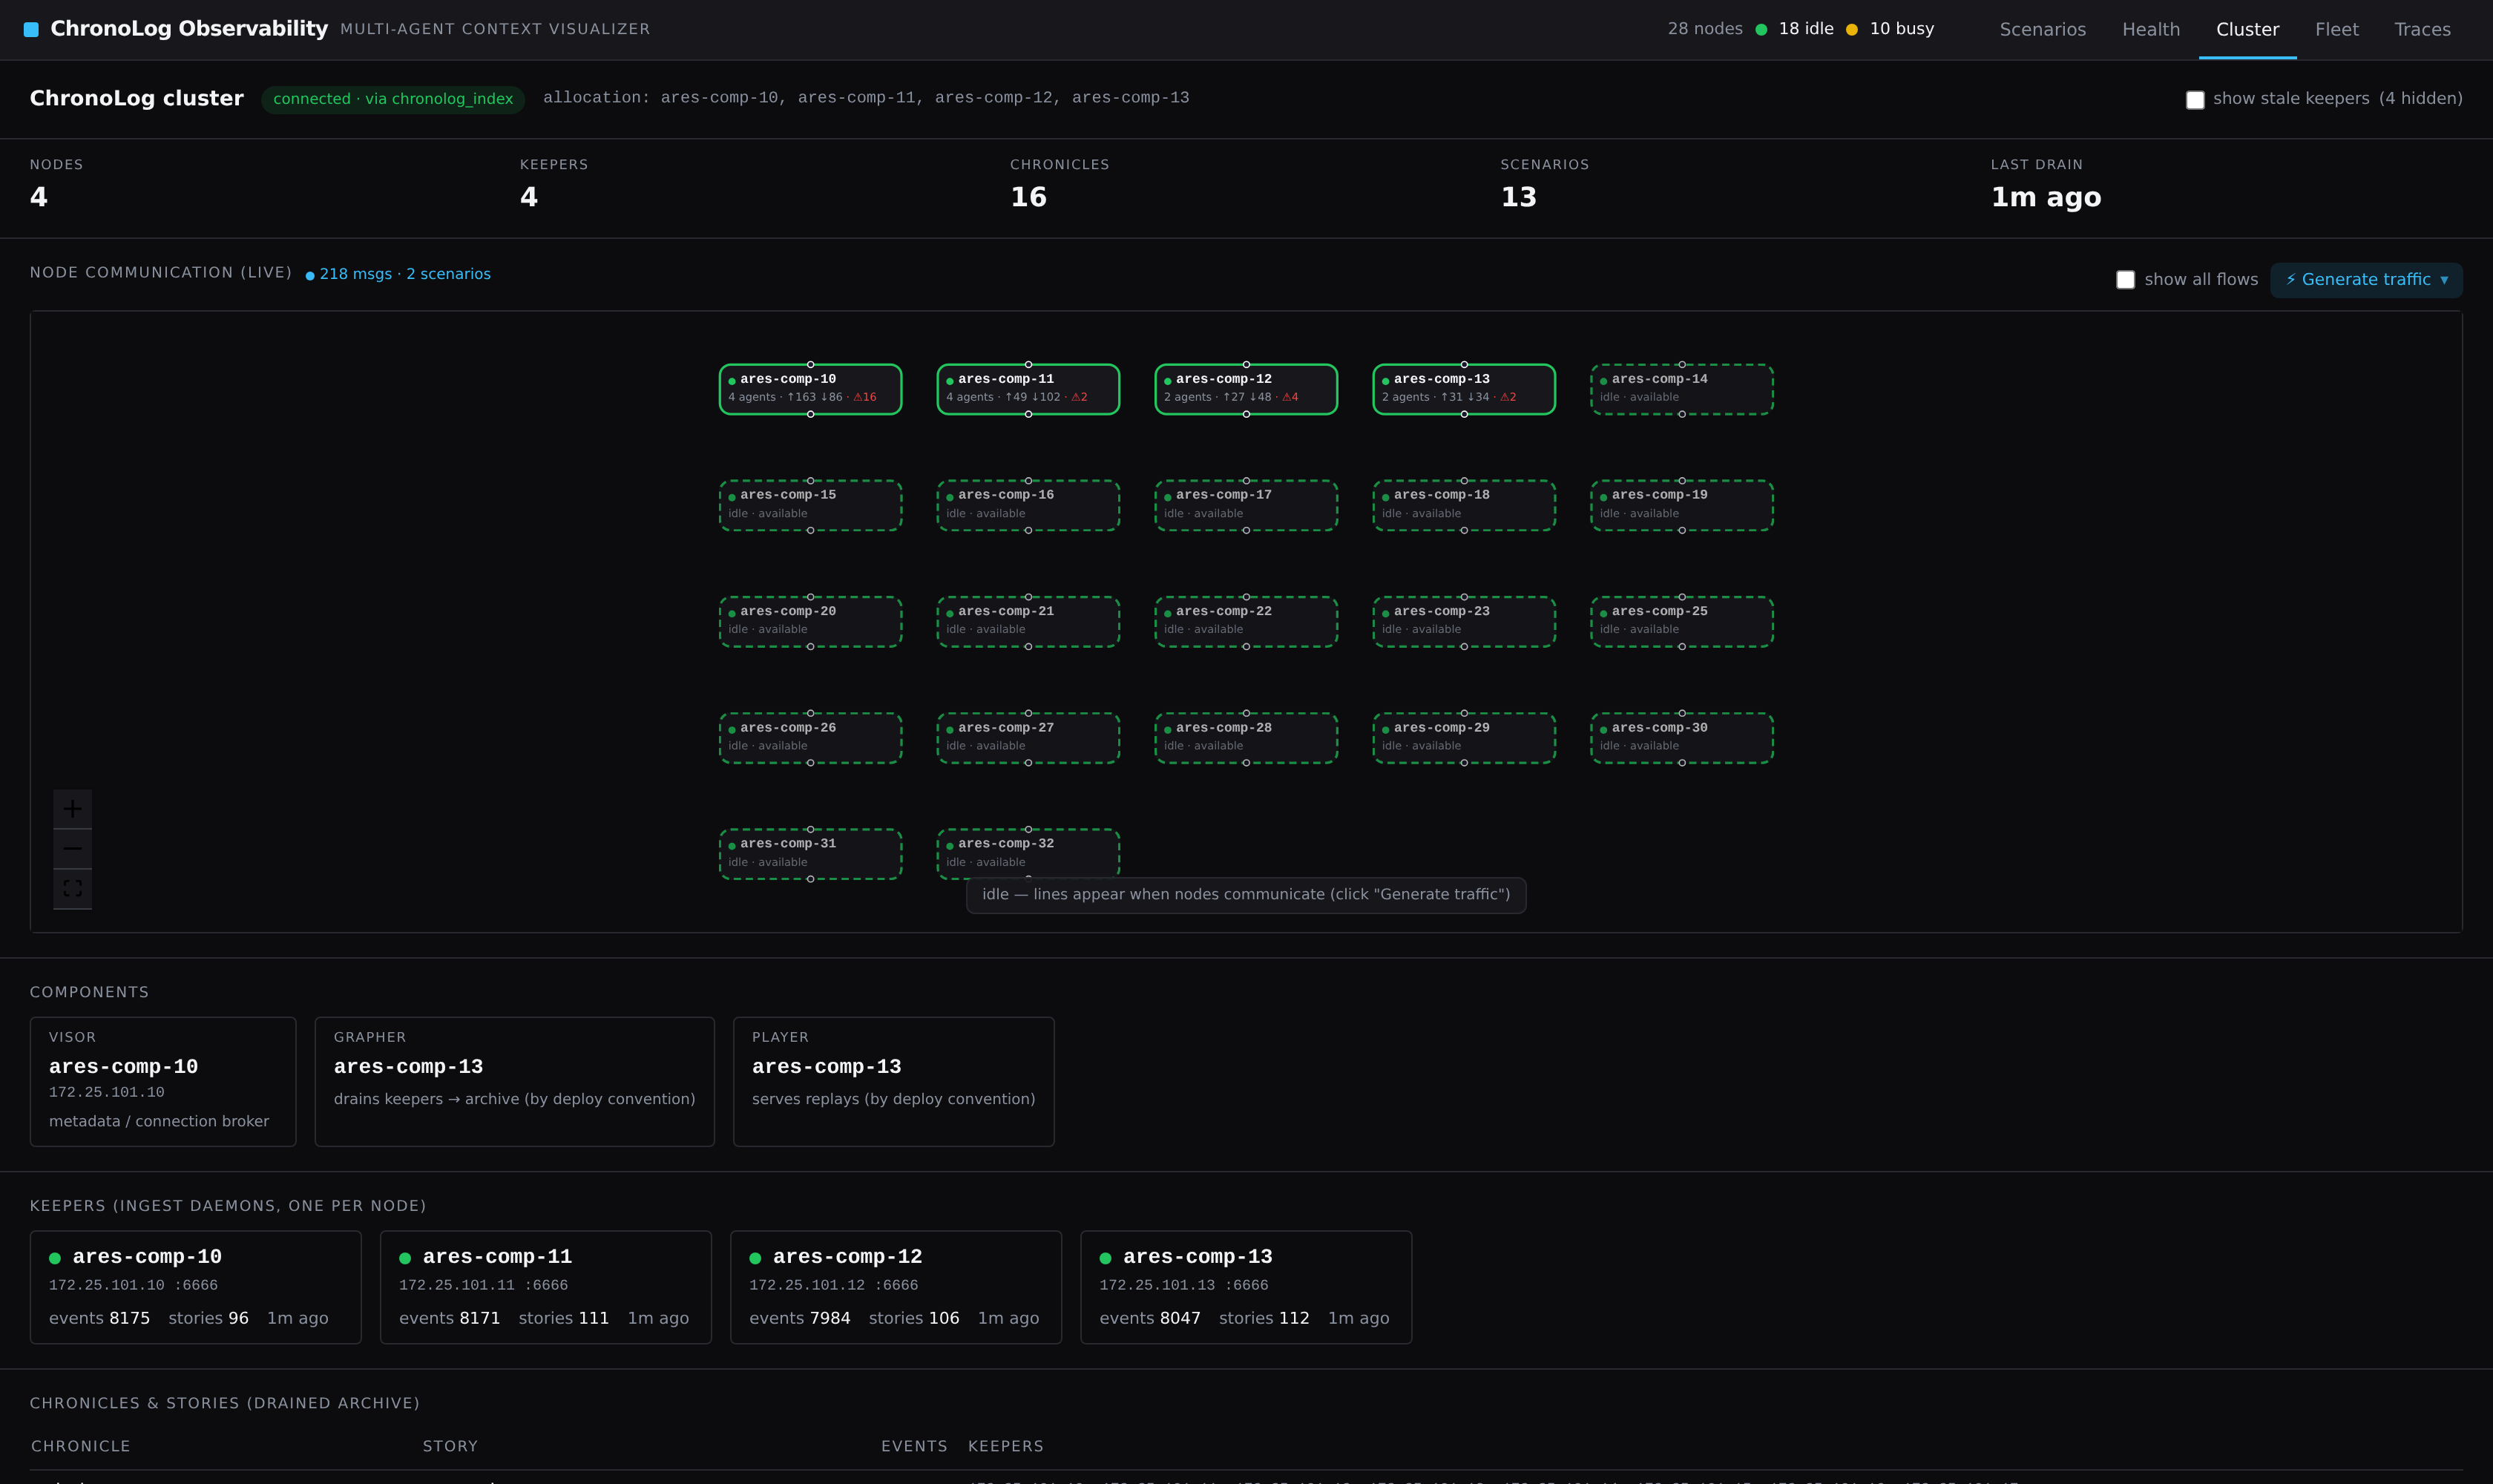
\includegraphics[width=\linewidth]{figures/ui-cluster}
  \caption{The Cluster view on a live 4-node deployment: ChronoLog
  components (visor, grapher, player placement; one keeper card per
  node with its event and story counts and last-drain age) alongside
  the live cluster graph and SLURM capacity. The headline
  freshness stat reports the \emph{measured} last-drain age
  (\S\ref{sec:eval-freshness}); the grapher's configured 180\,s
  acceptance window is relegated to its tooltip.}
  \label{fig:ui-cluster}
\end{figure}

\paragraph{Fleet: the population at a glance
(Fig.~\ref{fig:ui-fleet}).} One cell per node, colored by rolled-up
health state (ok / warn / crit, idle and busy dimmed), worst first;
the header aggregates events, errors, and cost over the selected
window. The representation change argued in
\S\ref{sec:analytics-fleet} pays off here: where the node-link graph saturates at a
dozen nodes, the heatmap stays legible at hundreds (the capture
below shows 256), and the red cells are the Q4 answer before a single
query is typed. Clicking a cell filters the fleet to that node and
hands off to the other views for the why.

\begin{figure}[p]
  \centering
  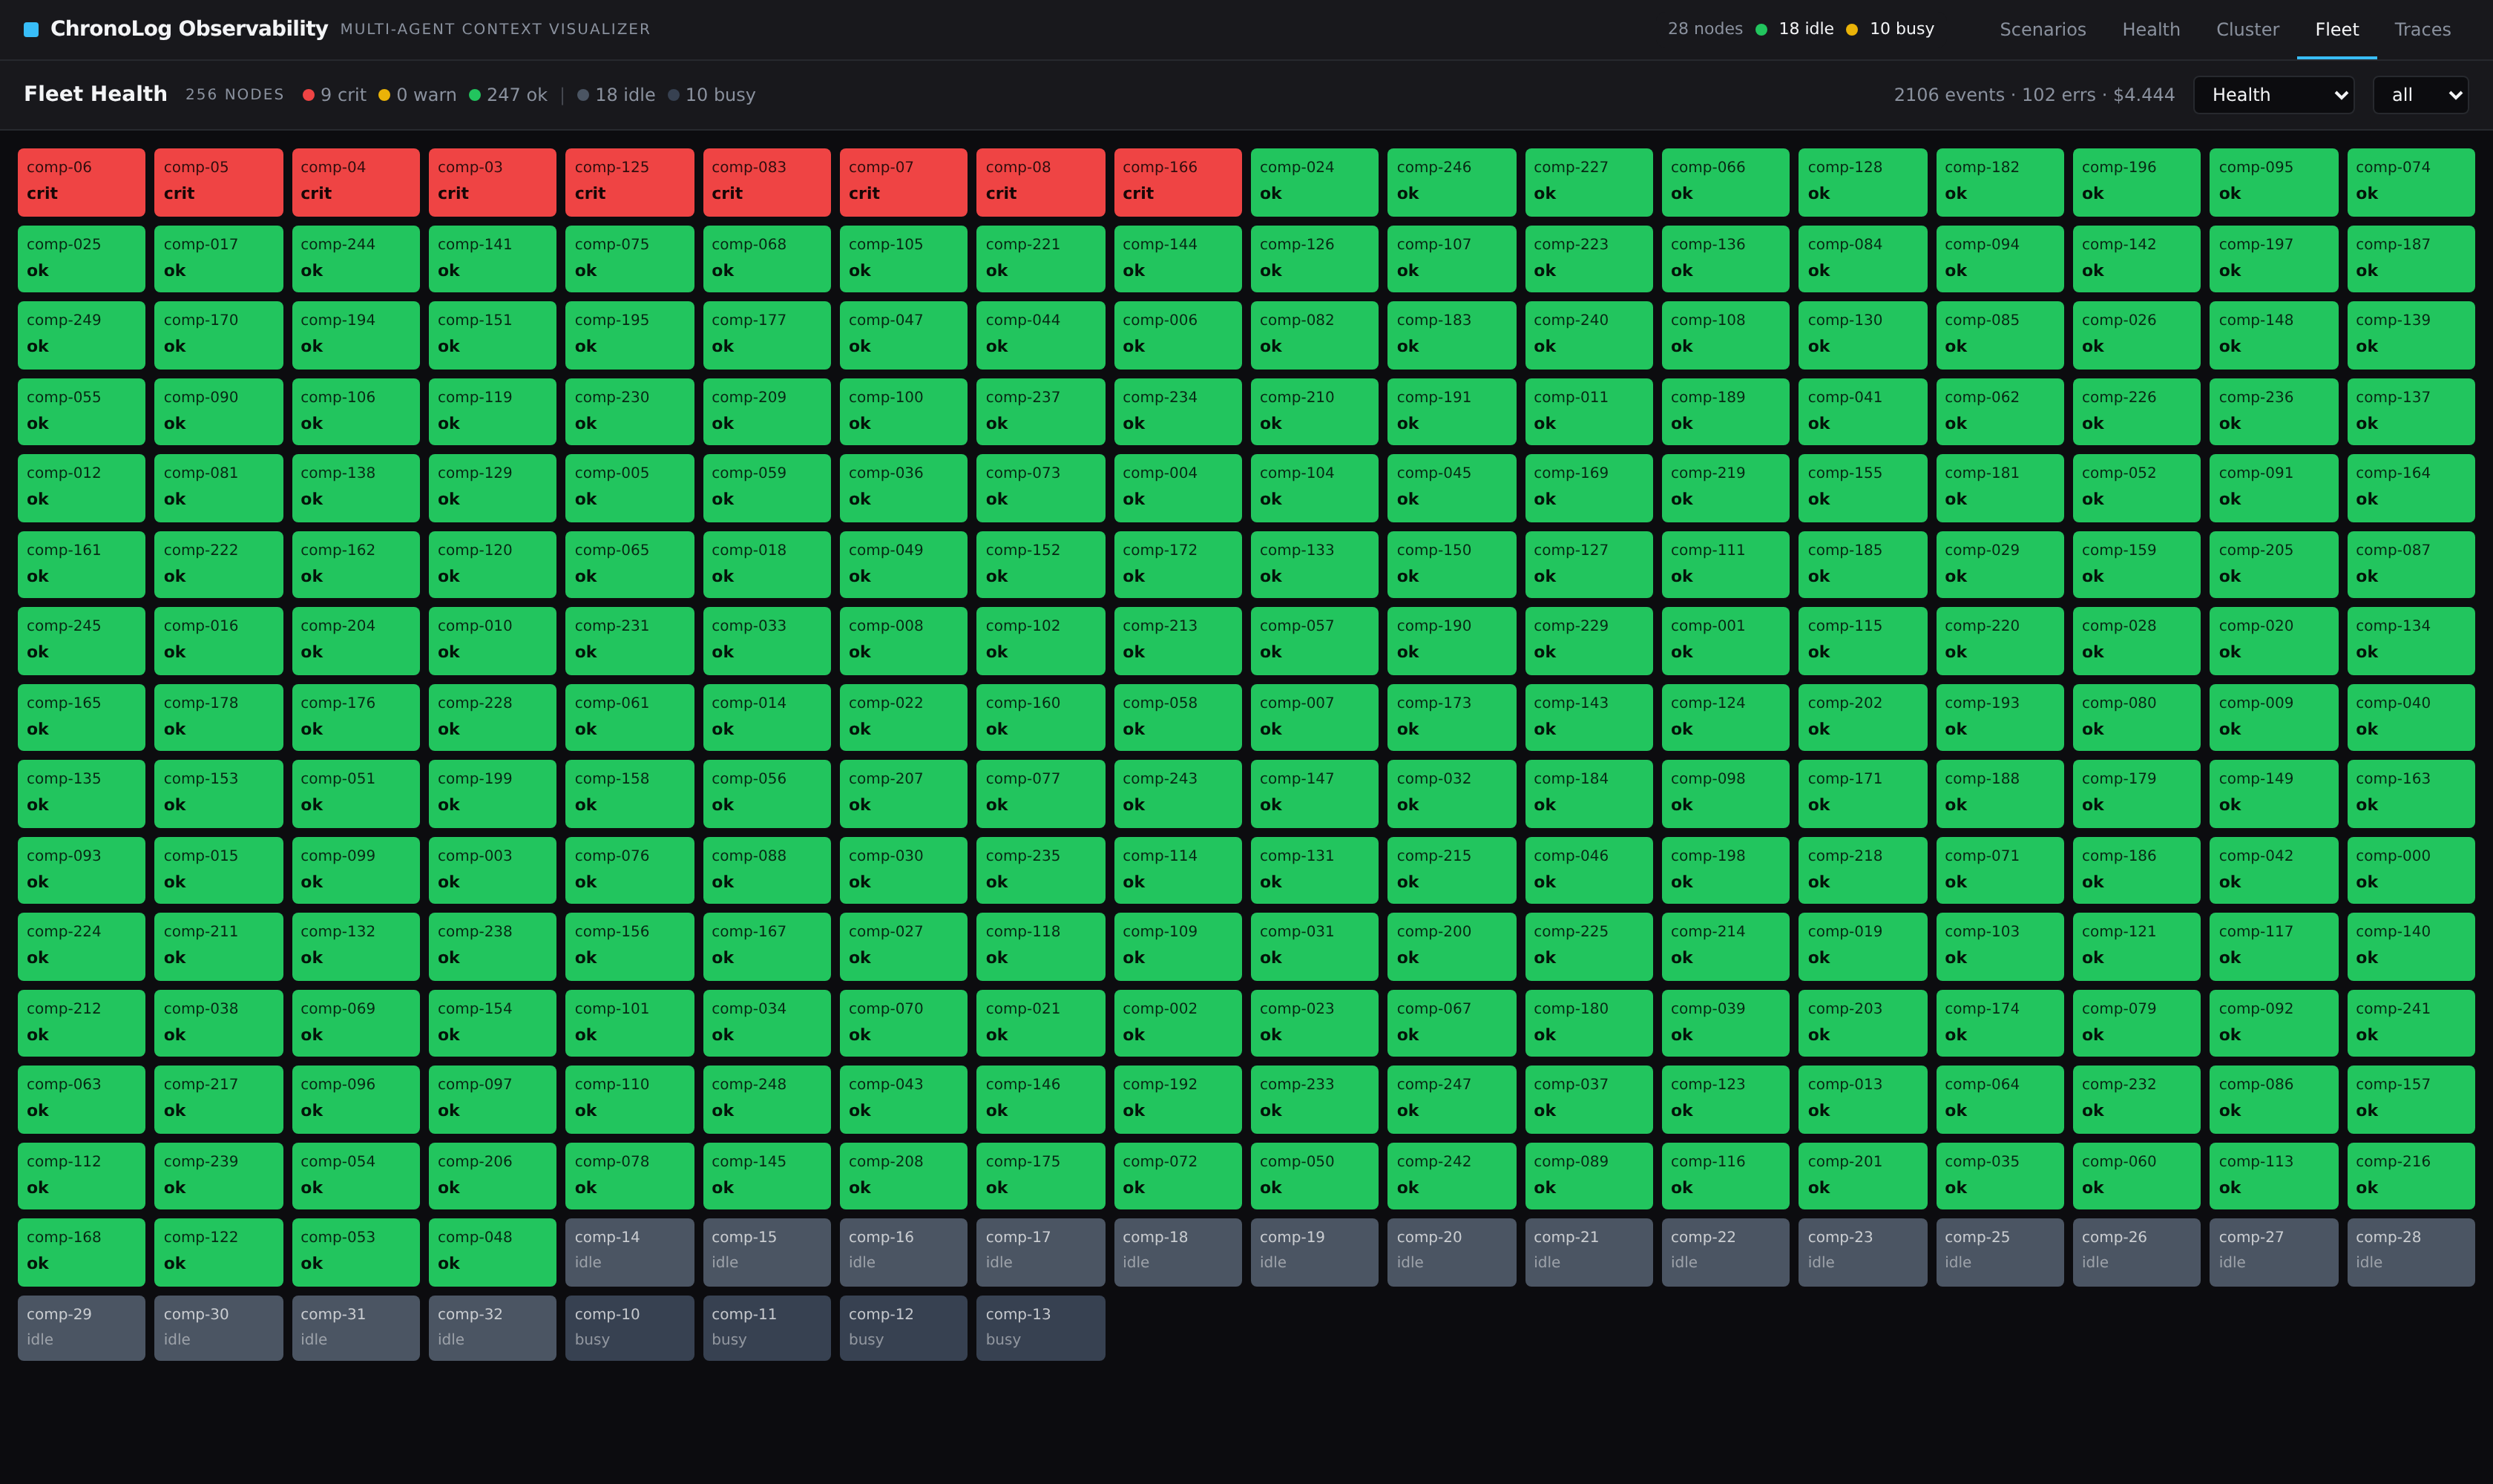
\includegraphics[width=\linewidth]{figures/ui-fleet}
  \caption{The Fleet view: 256 nodes, one cell each, rolled-up health
  worst-first. Nine critical nodes are the immediate Q4 answer.
  Rollup-backed reads keep this view interactive independent of event
  volume (\S\ref{sec:eval-scalability}).}
  \label{fig:ui-fleet}
\end{figure}

\paragraph{Traces: where the time went
(Fig.~\ref{fig:ui-traces}).} The critical-path surface of
\S\ref{sec:analytics-tracing}: traces listed slowest-first; the
selected trace rendered as a depth-indented waterfall with the critical
path outlined and each hop labeled \emph{tool $\to$ host}; the header
names the bottleneck hop with its self-time: in the capture,
\texttt{call\_remote\_agent} $\to$ \texttt{comp-04} at 12.0\,s of a
21.6\,s trace. A self-time bar above the waterfall shows at a glance
which host consumed the wall-clock, and clicking any span opens the
edge's detail. This is Q3 answered as a sentence, not a scroll.

\begin{figure}[p]
  \centering
  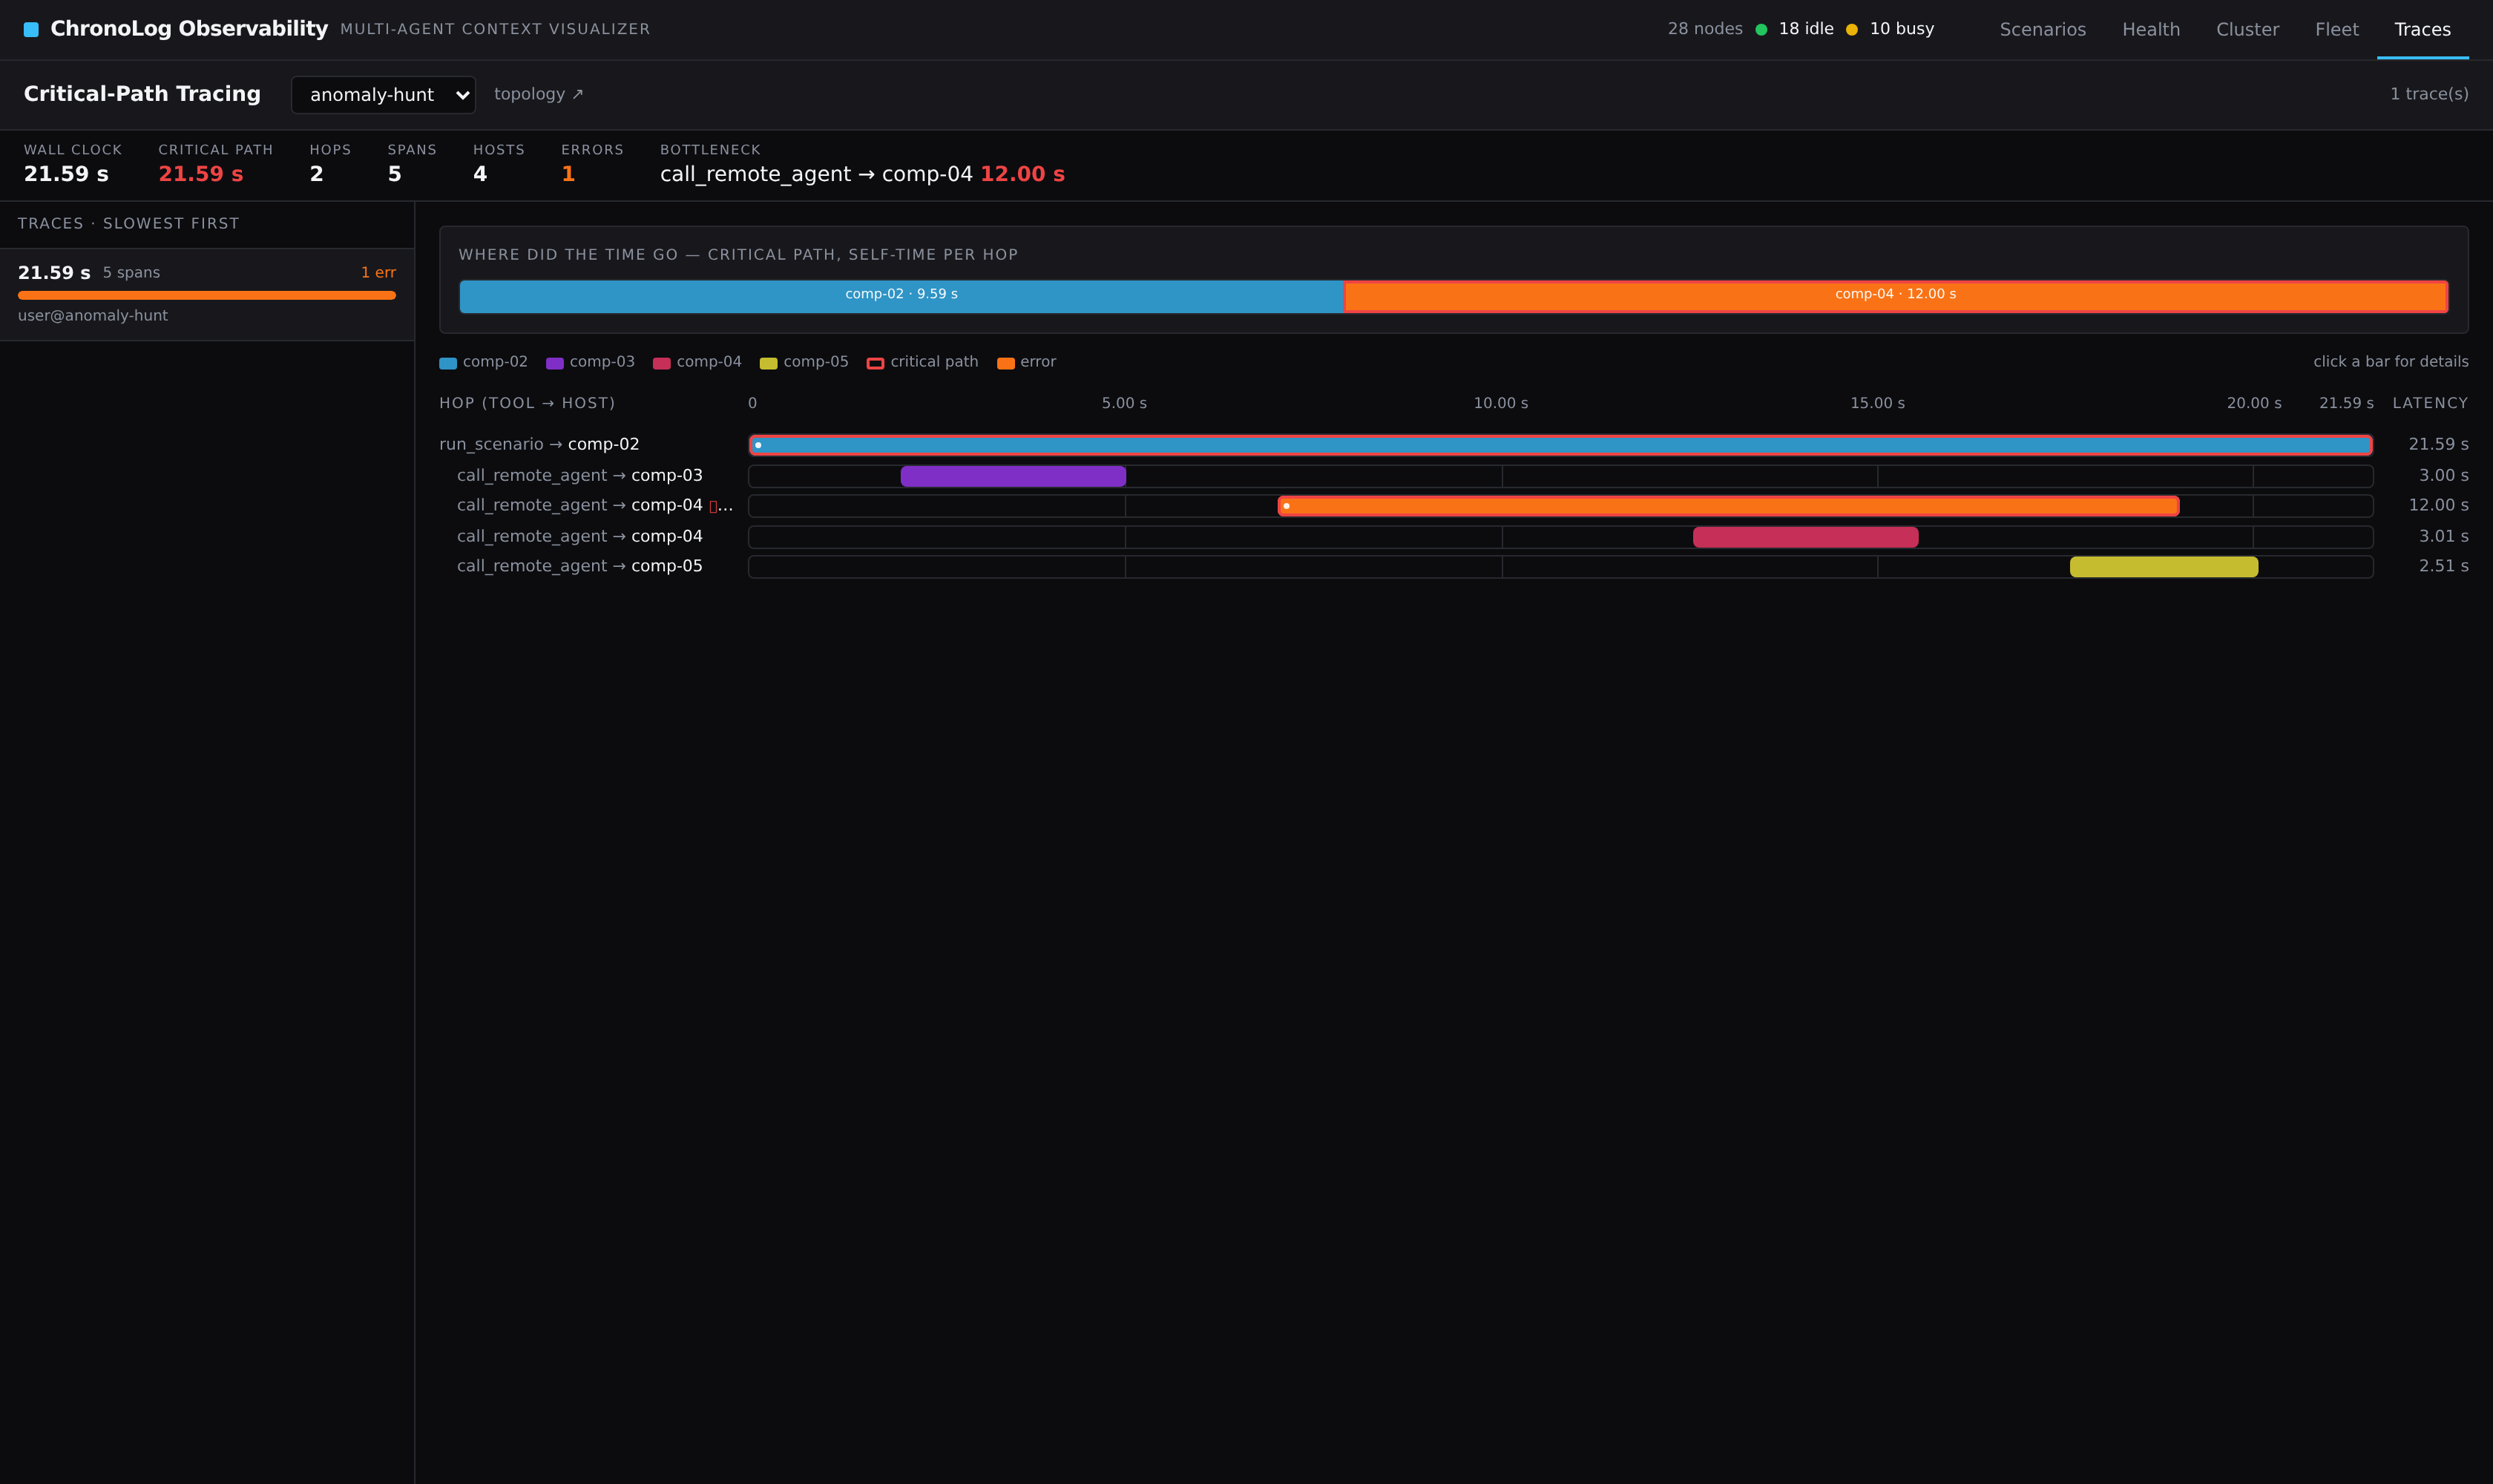
\includegraphics[width=\linewidth]{figures/ui-traces}
  \caption{The Traces view: critical-path waterfall for the slowest
  trace of a scenario. The header names the bottleneck (the
  \texttt{comp-04} hop, 12.0\,s self-time of 21.6\,s wall-clock); the
  top bar shows self-time per hop along the critical path.}
  \label{fig:ui-traces}
\end{figure}

Together the five views implement the pivot the case study of
\S\ref{sec:eval-casestudy} times end-to-end: Fleet says \emph{which
machine}, Health says \emph{what and why}, Traces says \emph{where the
time went}, Scenarios says \emph{who}, and the conversation view says
\emph{show me}. All are projections of one shared log, reachable from
each other in a click or two.

\chapter{Evaluation}
\label{chap:evaluation}

% All numbers are measured; raw data and scripts: scripts/eval/ and
% scripts/eval/out/ in the repository (summary.csv is the machine index).
% Live measurements: ARES, 8-node ChronoLog deployments, 2026-07-30/31.

The evaluation asks six questions, mapped to the requirements of
\S\ref{sec:problem-requirements}: what does capture cost the observed
workload (R5, \S\ref{sec:eval-overhead}); how fresh are the live views
(R2, \S\ref{sec:eval-freshness}); is the Doctor's diagnosis
\emph{correct}, not merely cheap (R6, \S\ref{sec:eval-doctor}); do the
analyses scale as claimed (R4,
\S\ref{sec:eval-scalability}); does the whole stack work end-to-end on a
real cluster with real agents (R1, R3, R7,
\S\ref{sec:eval-functional}); and does the system actually shorten the
path from symptom to cause (\S\ref{sec:eval-casestudy}).
Section~\ref{sec:eval-limitations} discusses limitations.
Table~\ref{tab:eval-glance} previews the headline results.

\begin{table}[t]
\centering
\small
\begin{tabular}{@{}p{0.34\linewidth}p{0.58\linewidth}@{}}
\toprule
\textbf{Question} & \textbf{Measured answer} \\
\midrule
What does capture cost the agent? &
  It adds $3.6$\,ms to a turn that averages $7.7$\,seconds, under
  $0.05\%$. Run against real agents with capture on and off, the
  difference was too small to measure (\S\ref{sec:eval-overhead}). \\
How fresh are the live views? &
  An event reaches the operator's screen in $10.7$\,ms. The durable
  archive takes $20$--$30$\,s to catch up, so the live view is roughly
  $1\,900\times$ faster (\S\ref{sec:eval-freshness}). \\
Is the diagnosis correct? &
  It found all $580$ planted faults and raised no false alarms on clean
  data. Five hundred identical errors were presented as one ranked
  incident (\S\ref{sec:eval-doctor}). \\
Do the analyses scale? &
  Fleet queries stayed at $19$--$24$\,ms while stored events grew
  $50\times$, and grow linearly with fleet size: $49$\,ms at 400 nodes
  of synthetic state (\S\ref{sec:eval-scalability}). \\
Does it run for real? &
  The whole stack passed all $28$ end-to-end checks on live 4- and
  8-node clusters, running up to $32$ real agents without per-node cost
  rising (\S\ref{sec:eval-functional}, \S\ref{sec:eval-scalability}). \\
Does it shorten diagnosis? &
  An operator meeting the fault for the first time diagnosed it
  completely in $72$\,seconds. From the raw logs the same operator could
  not answer any of the three questions (\S\ref{sec:eval-casestudy}). \\
\bottomrule
\end{tabular}
\caption[The evaluation at a glance]{The evaluation at a glance. Every number is measured; the
sections referenced give conditions, distributions, and caveats.}
\label{tab:eval-glance}
\end{table}

\section{Methodology}
\label{sec:eval-method}

\paragraph{Platform.} All live experiments run on the ARES cluster under
SLURM. Each experiment allocates $M$ idle compute nodes and deploys
ChronoLog across them (visor, one keeper per node, grapher draining to
an archive on shared storage), followed by the observability components:
one collector and one capture-worker process per node, and one dashboard
on a designated node. The deployments evaluated live use $M = 4$ and
$M = 8$. In this configuration the keeper seals 10\,s story chunks under a
15\,s acceptance window, while the grapher and player run with a
180\,s acceptance window; \S\ref{sec:eval-freshness} measures what these
settings translate to end-to-end, and corrects a folklore number in the
process.

\paragraph{Workloads.} Two workloads exercise the identical ingest path.
\emph{Real agents}: Claude Agent SDK agents, one or more per node
(configurable as $K$ agents per node), each performing genuine LLM turns
and one cross-node delegation through a remote-agent MCP tool per
round; turns enter Path-A, edges Path-B. \emph{Synthetic traffic}: a
generator that emits realistic interaction records and
\texttt{start}/\texttt{done} edge pairs through the same spool and
collector endpoints, with configurable topology (mesh, star, pipeline,
ring), agent count, node spread, error rate, and pacing. Real agents
provide ground truth end-to-end; synthetic traffic provides controlled,
reproducible, zero-token-cost load for overhead and scalability
measurements, and is the fault-injection vehicle for
\S\ref{sec:eval-casestudy}.

\paragraph{Measurements.} Latency overhead is measured as the difference
in per-turn wall-clock between instrumented and uninstrumented runs of
the same agent workload; capture-side costs by sampling the sidecar
processes' CPU and resident memory under load; storage by bytes per
record in each tier; freshness by timestamping an event at emission and
at receipt in a subscribed SSE client. Each is reported with distribution
statistics over repeated runs rather than as a single number: the workload
under test is a non-deterministic one running on shared cluster hardware,
which is exactly the regime in which single-run comparisons are known to
mislead, and in which a difference must be stated with a confidence
interval or not stated at all~\cite{georges2007rigorous}. Percentiles
rather than means are reported wherever an operator's experience is
governed by the tail~\cite{dean2013tail}.

\section{Capture Overhead}
\label{sec:eval-overhead}

Capture overhead is the cost the observed workload pays, and the design
predicts it is small by construction: the Path-A fast path is one local
JSONL append (no network, no lock, no downstream dependency,
\S\ref{sec:design-write}); the Path-B fast path is one HTTP POST to a
daemon on \texttt{localhost} that enqueues and returns. Both are
constant-time and independent of history size. Everything else (the
ChronoLog write, the forward, the drain) happens in sidecar processes
off the agent's critical path.

Figure~\ref{fig:capture-overhead} shows what capture adds to each event on
the agent's critical path, and Table~\ref{tab:overhead} the standing
resource and storage costs that a latency plot cannot show. All latency
numbers are taken on live compute nodes with the production NFS state
directory: the real deployment condition, not a tmpfs microbenchmark.

\begin{figure}[h]
  \centering
  % Capture overhead per event, by path (E1a/E1b; see tab:overhead for the
% resource and size rows). \input this inside a figure environment;
% needs \usepackage{pgfplots}.
%
% Data: scripts/eval/out/e1a_spool_latency_compute.csv (spool),
%       e1b_emit_collector.csv (collector), e1b_emit_fallback.csv (fallback);
% p50/p95 recomputed from those files and cross-checked against results.md.
%
% NOTE: the category names are used directly as the symbolic y coordinates.
% Do NOT reintroduce a separate `yticklabels={...}` list: with `ytick=data`
% pgfplots orders ticks by their order of appearance in the coordinate list,
% not by the `symbolic y coords` declaration, so a separate label list
% silently attaches the wrong name to each bar.
\begin{tikzpicture}
\begin{axis}[
    width=0.80\linewidth, height=4.8cm,
    xbar, bar width=7pt,
    xlabel={added latency per event (ms)},
    xmin=0, xmax=17,
    symbolic y coords={{Path-B fallback},{Path-B collector POST},{Path-A spool append}},
    ytick=data,
    yticklabel style={font=\small},
    nodes near coords, nodes near coords align={horizontal},
    every node near coord/.append style={font=\scriptsize, text=black},
    legend pos=north east, legend cell align=left,
    legend style={font=\small, draw=gray!40, fill=white, fill opacity=0.9,
                  text opacity=1},
    grid=major, grid style={dashed,gray!25},
    enlarge y limits=0.32,
    axis lines*=left,
    tick style={draw=gray!50},
]
\addplot[fill=gray!30, draw=gray!65, mark=none] coordinates {
    (0.83,{Path-A spool append})
    (2.82,{Path-B collector POST})
    (8.95,{Path-B fallback})};
\addplot[fill=gray!70, draw=gray!85, mark=none] coordinates {
    (1.09,{Path-A spool append})
    (6.22,{Path-B collector POST})
    (12.75,{Path-B fallback})};
\legend{p50, p95}
\end{axis}
\end{tikzpicture}

  \caption[Capture overhead per event, by path]{What capture adds to the
  agent's critical path, per event ($n{=}10\,000$ per bar, live 8-node
  deployment, production NFS state directory). Path-A's spool append is a
  local file write and costs under a millisecond. Path-B's POST to the
  node-local collector costs a few. The bottom pair is the degraded mode
  taken when the collector is down: the agent posts directly to the
  dashboard, at roughly $3\times$ the cost. Degradation is slower, not
  cheaper, which is why the collector exists. For scale, the mean LLM turn
  these sit inside is $7\,734$\,ms, three orders of magnitude to the right
  of this axis.}
  \label{fig:capture-overhead}
\end{figure}

\begin{table}[h]
\centering
\small
\begin{tabular}{@{}lllr@{}}
\toprule
\textbf{Cost} & \textbf{Path} & \textbf{Metric} & \textbf{Measured} \\
\midrule
\textbf{End-to-end turn delta} & A{+}B & instrumented vs.\ not, per turn &
  \textbf{$+365 \pm 2\,398$\,ms} \\
Collector daemon      & B & CPU / RSS per node, 20\,ev/s     & 32\% / 40\,MB \\
Capture worker        & A & CPU / RSS per node, same load    & 0.8\% / 51\,MB \\
Interaction record    & A & bytes per event (spool / archive) & 2\,093 / 2\,173\,B \\
Edge event            & B & bytes per event (hot / archive)   & 612 / ${\approx}560$\,B \\
Live forward          & B & bytes per event on the wire       & 646\,B \\
\bottomrule
\end{tabular}
\caption[Capture overhead: standing costs]{The standing costs of capture,
alongside the per-event latencies of Figure~\ref{fig:capture-overhead}
(live 8-node deployment, compute nodes, NFS state directory).
The first row is the end-to-end A/B turn delta over real LLM turns:
its 95\% confidence interval spans zero, so capture is statistically
invisible inside the workload's own variance. Capture worker CPU is the
mean of a bursty profile (idle between 5\,s drain passes, peaks of 85\%
during them); the wire number is amortized over batches of ${\le}64$
(658\,B unbatched).}
\label{tab:overhead}
\end{table}

The headline is easy to over- and under-claim, so it needs stating
carefully. The A/B experiment ran $n{=}30{+}30$ real agent turns
(identical prompts, interleaved to absorb provider drift): instrumented
turns averaged $8\,099 \pm 5\,147$\,ms, uninstrumented
$7\,734 \pm 4\,291$\,ms, a delta of $+365$\,ms whose 95\% confidence
interval ($\pm 2\,398$\,ms, Welch $t = 0.30$) makes it statistically
indistinguishable from zero. The claim therefore rests on both
measurements: the \emph{mechanism} costs
$0.83 + 2.82 \approx 3.6$\,ms per turn-plus-delegation (under
\textbf{0.05\%} of a 7.7\,s mean turn), and the A/B run confirms that
nothing beyond the mechanism leaks onto the critical path. With the
collector \emph{down}, the fallback POST to the dashboard costs
$3\times$ the normal path (8.95 vs.\ 2.82\,ms p50): degraded mode is
slower, not cheaper, which is why the collector exists.

Two structural observations frame the numbers. First, the denominator is
large: an LLM turn takes seconds and a delegation round-trip longer, so
capture cost in milliseconds translates to a per-turn overhead orders of
magnitude below the workload's own variance. This is the inverse of the
classical tracing regime (\S\ref{sec:bg-sampling}), where sub-millisecond
RPCs made even microseconds of instrumentation significant; it is
why complete capture is affordable here. Second, the failure-mode cost is
bounded by design rather than measured luck: if every downstream component
dies, the agent's cost is unchanged (Path-A) or one failed local
connection followed by a fallback POST (Path-B).

\section{Freshness and Query Latency}
\label{sec:eval-freshness}

Freshness is the interval from an agent emitting an event to that event
being visible to an operator. The claim under test is that the hot path
(R2) puts the event on screen in milliseconds while the cold path
delivers durability in tens of seconds, and the measurement corrects a
number this thesis itself repeated from deployment folklore.

Figure~\ref{fig:query-latency} plots the whole range on one axis: the
hot-path pipeline (emit $\to$ collector $\to$ dashboard ingest $\to$ SSE
frame at a subscribed client), each per-view query against the populated
live deployment, and the cold-path drain they must all be read against.
Four numbers do not fit on that axis and are given in
Table~\ref{tab:freshness}: the tails, the degraded path, and the
rollup-backed fleet read that \S\ref{sec:eval-scalability} explains.

\begin{table}[h]
\centering
\small
\begin{tabular}{@{}llr@{}}
\toprule
\textbf{Measure} & & \textbf{Measured} \\
\midrule
Emit $\to$ SSE frame at client   & p95          & 11.8\,ms \\
\quad direct-ingest fallback     & p50 / p95    & 8.5 / 8.9\,ms \\
Cold-path availability (drain)   & max, $n{=}10$ & 30\,s \\
Fleet health, rollup-backed (\S\ref{sec:eval-scalability}) & p50 & 19--24\,ms \\
\bottomrule
\end{tabular}
\caption[Freshness and query latency: tails and degraded paths]{The
freshness numbers Figure~\ref{fig:query-latency} cannot show: the tail of
the live push, the degraded direct-ingest path taken when the collector is
down, the worst drain observed, and the rollup-backed fleet read.
Live 8-node deployment, dashboard node, $n{=}100$ per query row,
$n{=}1\,000$ paced events at 20\,ev/s with zero loss for the SSE rows,
corpus ${\approx}22$\,k archived events.}
\label{tab:freshness}
\end{table}

\begin{figure}[t]
  \centering
  % Freshness / query latency spread, one log axis (p50, live 8-node run).
% Data: scripts/eval/out/summary.csv (E2a live, E2c live rows).
\begin{tikzpicture}
\begin{axis}[
    xbar,
    xmode=log,
    log origin=infty,
    width=0.62\linewidth,
    height=5.6cm,
    xmin=1, xmax=300000,
    xtick={1,10,100,1000,10000},
    xticklabels={1,10,100,$10^3$,$10^4$},
    xlabel={p50 latency (ms, log scale)},
    symbolic y coords={
      {Cold-path drain},
      {Cluster graph},
      {Fleet health (raw)},
      {Doctor scan},
      {Scenario graph},
      {Trace rebuild},
      {Live push}},
    ytick=data,
    y dir=normal,
    yticklabel style={font=\small},
    xticklabel style={font=\small},
    xlabel style={font=\small},
    nodes near coords,
    nodes near coords style={
      font=\scriptsize, anchor=west, xshift=2pt},
    point meta=explicit symbolic,
    bar width=7pt,
    enlarge y limits=0.12,
    axis lines*=left,
    tick style={black},
]
\addplot[fill=black!25, draw=black!60] coordinates {
  (10.7,{Live push}) [10.7\,ms]
  (282,{Trace rebuild}) [282\,ms]
  (470,{Scenario graph}) [470\,ms]
  (1807,{Doctor scan}) [1.8\,s]
  (1881,{Fleet health (raw)}) [1.9\,s]
  (2009,{Cluster graph}) [2.0\,s]
  (20000,{Cold-path drain}) [20\,s]
};
\end{axis}
\end{tikzpicture}

  \caption[Freshness and query latency, measured]{The freshness and query-latency spread on one log axis (p50,
  live 8-node deployment). Live push takes single-digit milliseconds and
  scenario-scoped reads stay sub-second, while population-wide reads
  that fold the raw archive sit near $2$\,s on this corpus. That is the
  linear-in-events cost the rollup design of
  \S\ref{sec:eval-scalability} flattens to roughly $20$\,ms.}
  \label{fig:query-latency}
\end{figure}

\paragraph{The drain is 20--30\,s; the ``$\sim$180\,s'' was something
else.} Measured directly (append a marked event, poll the archive), a
story chunk becomes readable \textbf{20--30\,s} after append ($n{=}10$,
p50 20\,s), governed by the keeper's 10\,s chunking and 15\,s
acceptance window plus the grapher's write batch, not by the 180\,s
window configured downstream. The ${\sim}180$\,s that operators (and
earlier drafts of this thesis) attributed to the drain is in fact the
client's \emph{replay-query timeout}. In these deployments the player's
playback responses never reach the dashboard process's receiver
service: the player logs every request and completes none of the
transfers toward that endpoint, while an otherwise-identical receiver
in the capture process works. Every live replay issued by the dashboard
therefore blocks for the full \texttt{CL\_ERR\_QUERY\_TIMED\_OUT}
window of ${\sim}180$\,s: per story, per request, holding the client
lock.
Diagnosing this (\S\ref{sec:eval-limitations}) explained the
folklore number and motivated generalizing the archive-first read rule
of \S\ref{sec:design-read} from listing indexes to \emph{all} dashboard
replays: with the drain at 20--30\,s, serving full-fidelity views from
the archive costs at most half a minute of staleness and removes the
last blocking read from the serving process.

Qualitatively, the split then behaves as designed in every live run: the
live views (scenarios, cluster, fleet, health, traces) render
immediately during a run, while full-fidelity conversation views fill in
within the half-minute drain; no view blocks the dashboard, fresh
clusters included.

\section{Detection Quality}
\label{sec:eval-doctor}

R6 demands that diagnosis be free of marginal token cost; this section
asks whether the deterministic pipeline that satisfies it is also
\emph{correct}. The experiment scores a full Doctor scan (gather,
detect, cluster, diagnose, record; \S\ref{sec:analytics-doctor})
against a ground-truth manifest of
injected faults. Deliberately injecting the failure and checking that the
system reports it is the discipline of controlled fault
injection~\cite{basiri2016chaos}, applied here offline rather than in
production so that the manifest is exact and the false-positive rate is
measurable against a known-clean background.
A controlled corpus is seeded offline through the same
spool and inter-agent-store write paths the capture layer uses: a clean
background of healthy traffic (216 turns, 120 completed delegations),
plus ten planted faults of each of the eight detector families of
\S\ref{sec:analytics-doctor} (5xx errors, rate-limiting, retry storms,
latency outliers, edge errors, orphan calls, slow edges, recoveries),
plus one \emph{storm} (500 identical peer-timeout edges spread across 40
hosts) to test that section's compression claim. Each planted fault is
shaped to carry exactly one symptom (single-label ground truth), so every
detection is unambiguously attributable. The same fault mix is then
injected a second time and the corpus re-scanned, testing whether the
incident history recognizes the recurrence.

The result is a clean sweep: all 580 planted signals were detected, the
eighty single faults and every event of the storm alike, and every
incident was routed to its intended diagnosis rule, at confidences from
0.55 (latency outliers, slow edges) to 0.85 (rate limiting). The scan is
seed-deterministic (\texttt{e6\_doctor\_\allowbreak quality.py} in
\texttt{scripts/eval/}), and the result is identical at $n{=}25$ and
under a different seed.

Three results carry the argument. First, the clean background
produces \emph{zero} incidents: the detectors' thresholds (medians with
absolute floors, consecutive-repeat minima) do not fire on healthy
variance, so a ranked incident list starts empty rather than requiring
the operator to learn a noise floor. Second, compression behaves as
designed: 580 injected raw signals become 9 ranked incident cards;
in particular the 500 identical timeouts collapse into \emph{one} card
whose count, host list, and severity escalation carry the blast radius
(the ``not a scroll of per-event errors'' the operator asked for). Third,
the longitudinal claim holds mechanically: after the first scan writes the incident
memory, the second scan badges all nine incidents as recurring with the
correct prior count, read back from the self-compacting memory document
rather than from process state.

The scope of the claim is bounded. The planted faults are
in-distribution and comfortably above the detector thresholds: the
experiment establishes that detection, clustering, diagnosis routing,
and cross-run memory are correct on unambiguous faults, not that the
thresholds are well-calibrated on borderline cases. ``Diagnosis
correct'' likewise means only that the incident reached the intended
rule of the hand-built rule set, whose coverage limits are discussed in
\S\ref{sec:eval-limitations}. A perfect score under these conditions is
the expected behavior of deterministic detectors, not evidence against
harder inputs; the informative results are the zero-false-positive
background, the exact $500{\to}1$ compression, and the memory
round-trip.

\section{Scalability}
\label{sec:eval-scalability}

The evaluation tests three scaling claims.

\paragraph{Fleet reads are independent of event volume.} The rollup
design (\S\ref{sec:analytics-fleet}) makes the fleet query
$O(\text{nodes} \times \text{buckets})$; the raw-fold fallback is
$O(\text{events})$. The experiment holds nodes and window fixed (16
nodes, 60-minute window) and grows the event count from $10^4$ to
$5 \times 10^5$, comparing the fleet-health query latency of the two
paths (20 requests per point, p50). Figure~\ref{fig:rollup-scaling}
shows the result: rollup-backed reads stay flat at 19--24\,ms across a
$50\times$ growth in event volume, while the raw fold grows linearly
(slope ${\approx}17$\,ms per thousand events between the endpoints):
107\,ms at 10\,k events, 8.5\,s at 500\,k, a $457\times$ gap at the
largest size.

\paragraph{Fleet reads grow linearly in fleet size, and only in fleet
size.} The complementary experiment holds the per-node event density fixed
and grows the \emph{number of nodes}. It cannot be run on the live
allocation: the largest cluster available here was eight nodes
(\S\ref{sec:eval-functional}). It is therefore run against
\emph{synthetic fleet state}: the harness invents $n$ host names and
writes their events through the production capture API, the production
emitter bucketizes them, and the production dashboard is then queried over
HTTP exactly as an operator would. What is synthetic is the origin of the
events; the store, the query path and the measured latency are the real
ones. This is sufficient for the claim under test, which is a property of
the read algorithm: the fold cost depends on how many buckets exist, not on
which machine produced them. It is correspondingly \emph{not} evidence
about capture, drain or network behaviour at that scale, which the live
4- and 8-node deployments cover instead.

Figure~\ref{fig:fleet-nodes} shows the result over fleets of 10 to 400
nodes (50 requests per point). Latency is linear in node count,
$5.2 + 0.105n$\,ms with $R^2 = 0.98$: a fixed ${\sim}5$\,ms of request
handling plus ${\sim}0.1$\,ms per node summarized. A 100-node fleet is
answered in 14.7\,ms p50 and a 400-node fleet in 49.0\,ms, both inside
interactive time, where the same query folded from raw events would touch
every record ever captured. The 100-node point reproduces an
independent measurement taken on the cluster three weeks earlier
(15.1\,ms), which is the reason to trust the rest of the curve. The sweep
stops at 400 nodes because that is the emitter's configured session bound
(\texttt{max\_sessions}, \S\ref{sec:analytics-fleet}); beyond it the
harness silently re-measures a 400-node fleet rather than a larger one.

\begin{figure}[t]
  \centering
  \input{figures/fig-rollup-scaling}
  \caption[Fleet-query latency vs.\ stored event count]{Fleet-health query latency vs.\ stored event count (16 nodes,
  60-minute window, p50 over 20 requests). Pre-aggregated rollup reads
  are independent of event volume; the raw-fold fallback is linear in
  it. Measured offline via
  \texttt{bench\_rollup\_\allowbreak scaling.py} in
  \texttt{scripts/eval/}.}
  \label{fig:rollup-scaling}
\end{figure}

\begin{figure}[t]
  \centering
  % Fleet-health query latency vs. FLEET SIZE (E3b, re-measured 2026-08-10).
% Complements fig-rollup-scaling, which holds nodes fixed and grows events.
% \input this inside a figure environment; needs \usepackage{pgfplots}.
%
% Data: thesis/figures/e3b_heatmap_nodes_p50.csv, derived from
% scripts/eval/out/e3b_heatmap_nodes.csv (50 requests per point, synthetic
% fleet state, real dashboard, ARES gateway).
\begin{tikzpicture}
\begin{axis}[
    width=0.85\linewidth, height=6cm,
    xlabel={fleet size (nodes; synthetic rollup state)},
    ylabel={\texttt{/api/fleet/health} latency (ms)},
    xmin=0, xmax=420, ymin=0,
    legend pos=north west, legend cell align=left,
    legend style={font=\small, draw=gray!40},
    grid=major, grid style={dashed,gray!25},
    tick style={draw=gray!50},
]
\addplot[dashed, gray!70, domain=0:400, samples=2] {5.20 + 0.1053*x};
\addlegendentry{$5.2 + 0.105\,n$ (fit, $R^2{=}0.98$)}
% Styles set explicitly rather than taken from the cycle: the dashed fit line
% above consumes a cycle index, which would otherwise render p95 heavier than
% p50 and make the secondary series the visually dominant one.
\addplot[black!80, thick, mark=*, mark size=1.6pt,
         mark options={fill=black!30, draw=black!80}]
    table [x=nodes, y=p50_ms, col sep=comma]
    {figures/e3b_heatmap_nodes_p50.csv};
\addlegendentry{p50}
\addplot[black!45, thick, mark=square*, mark size=1.6pt,
         mark options={fill=black!8, draw=black!45}]
    table [x=nodes, y=p95_ms, col sep=comma]
    {figures/e3b_heatmap_nodes_p50.csv};
\addlegendentry{p95}
\end{axis}
\end{tikzpicture}

  \caption[Fleet-query latency vs.\ fleet size]{Fleet-health query latency
  vs.\ \emph{fleet size} (50 requests per point), the complement to
  Figure~\ref{fig:rollup-scaling}: there the node count is fixed and events
  grow, here events per node are fixed and the fleet grows. Latency is
  linear in nodes, $5.2 + 0.105n$\,ms ($R^2 = 0.98$).
  \textbf{The fleet state is synthetic}: the harness invents $n$ host names
  and writes their events through the production capture path, so the store,
  the query and the timings are real but no $n$-node cluster is involved.
  The largest \emph{live} deployment in this thesis is eight nodes
  (\S\ref{sec:eval-functional}). The sweep stops at 400 nodes, the emitter's
  configured session bound. Measured on the ARES gateway via
  \texttt{bench\_rollup\_\allowbreak scaling.py} in \texttt{scripts/eval/}.}
  \label{fig:fleet-nodes}
\end{figure}

\paragraph{Representation, not just computation, must scale.} The
node-link cluster graph is legible to roughly a dozen nodes and
degenerates beyond; this is a limit of the visual form, not of the
data. The fleet heatmap holds one cell per node and remains legible at
hundreds; its rendering cost grows with nodes only. This is why the
system changes representation between the topology view (small $M$, maximal
detail) and the population view (large $M$, one health value per node).

\paragraph{Agents per node.} The real-agent harness scales in two
dimensions: nodes ($M$) and agents per node ($K$). Capture is per-node
(one collector, one keeper, one worker regardless of $K$), so
per-node capture load grows linearly in $K$ with no cross-node
coordination, and cross-node load grows only with actual inter-agent
traffic. Live runs swept $K \in \{1, 2, 4\}$ at $M = 8$ with real agents
(every agent performing genuine LLM turns and one cross-node delegation):
all $8$, $16$, and $32$ agents exited cleanly and every delegation
round-tripped through the archive (16, 32, and 64 edge records
respectively). The per-node sidecar was flat across the sweep
(Figure~\ref{fig:agents-per-node}): the
collector held $0.1$--$0.3\%$ mean CPU (transient forward bursts to
${\sim}21\%$) and $37$--$39$\,MB RSS at every $K$, and the capture
worker $0.3\%$ mean at $48$\,MB. Neither series is monotonic in $K$: CPU
falls from $K{=}1$ to $K{=}2$ and rises again at $K{=}4$, which is
the signature of measurement noise around a constant rather than of a
trend, and is the result the design predicts: one collector, one keeper
and one worker serve a node whatever $K$ is. These means sit far below
Table~\ref{tab:overhead}'s 32\% figure because the regimes differ: the
table's collector serves a sustained 20\,ev/s synthetic stress load,
while real agents (one turn every several seconds) offer a small
fraction of that rate. Both observations are consistent with the claim
that agent count stresses the LLM provider, not the capture plane. The
largest configuration exercised cleanly end-to-end is therefore
$K {\times} M = 4 {\times} 8 = 32$ real agents.

\begin{figure}[h]
  \centering
  % Per-node sidecar load vs. agents per node (E3c, live 8-node sweep).
% Two separate axes rather than one with two y-scales: CPU (%) and RSS (MB)
% are different units, and a dual-axis plot would invite a false comparison.
% Both axes start at zero, so "flat" reads as flat rather than as an
% artefact of a truncated baseline.
%
% Data: scripts/eval/out/e1d_sidecars_k{1,2,4}.csv (collector process),
% cross-checked against the E3c table in scripts/eval/out/results.md.
\begin{tikzpicture}
\begin{axis}[
    width=0.46\linewidth, height=4.4cm,
    ybar, bar width=13pt,
    xlabel={agents per node ($K$)}, ylabel={collector CPU, mean (\%)},
    symbolic x coords={1,2,4}, xtick=data,
    ymin=0, ymax=0.5,
    nodes near coords, every node near coord/.append style={font=\scriptsize, text=black},
    grid=major, grid style={dashed,gray!25},
    tick style={draw=gray!50},
    enlarge x limits=0.35,
    title style={font=\small}, title={(a) CPU},
]
\addplot[fill=gray!45, draw=gray!75, mark=none] coordinates {(1,0.34) (2,0.13) (4,0.25)};
\end{axis}
\end{tikzpicture}
\hfill
\begin{tikzpicture}
\begin{axis}[
    width=0.46\linewidth, height=4.4cm,
    ybar, bar width=13pt,
    xlabel={agents per node ($K$)}, ylabel={collector RSS, mean (MB)},
    symbolic x coords={1,2,4}, xtick=data,
    ymin=0, ymax=50,
    nodes near coords, every node near coord/.append style={font=\scriptsize, text=black},
    grid=major, grid style={dashed,gray!25},
    tick style={draw=gray!50},
    enlarge x limits=0.35,
    title style={font=\small}, title={(b) Memory},
]
\addplot[fill=gray!45, draw=gray!75, mark=none] coordinates {(1,36.7) (2,39.0) (4,36.9)};
\end{axis}
\end{tikzpicture}

  \caption[Per-node capture load vs.\ agents per node]{Per-node capture load
  as agents per node quadruples, measured on the live 8-node sweep with real
  agents ($K \in \{1,2,4\}$, i.e.\ 8, 16 and 32 agents in total). Both axes
  start at zero, and neither quantity trends: the collector's mean CPU is
  non-monotonic in $K$ (noise around a constant, not growth) and its
  resident memory moves by ${\sim}2$\,MB across the sweep. This is the
  design's prediction (one collector, one keeper and one capture worker
  serve a node regardless of how many agents run on it), so adding agents
  costs the LLM provider, not the capture plane. CPU and memory are drawn on
  separate axes because they share no unit; the transient forward bursts to
  ${\sim}21\%$ are not shown, being spikes rather than sustained load.}
  \label{fig:agents-per-node}
\end{figure}

\section{Functional Validation}
\label{sec:eval-functional}

The system's end-to-end correctness claim, capture through the log store to
every view with real agents on a real cluster (R1, R3, R7), is
validated by an automated harness rather than by demonstration. The
harness brings up the full deployment on a live allocation, runs real
Claude agents (genuine LLM turns; one cross-node MCP delegation
per agent), waits out the drain, restarts the dashboard cold against the
same log store (so everything shown is reconstructed from durable state,
not process memory), and then asserts machine-checkable properties of
every API the dashboard serves: each view is populated with the expected
entities, per-agent metrics are non-zero where turns occurred, and
inter-agent edges exist with correct endpoints. The strictest check is
the cross-plane join: the scenario graph's clicked node resolves to that
agent's conversation with its turns and token counts, exercising the
session-identity contract of \S\ref{sec:design-mapping} end to end.

The harness passes \textbf{28/28} checks on live 4-node and 8-node
ChronoLog clusters. Beyond the pass count, the harness is the regression
suite the design was corrected against: the read-only rule, the archive-first
index read, and the hostname canonicalization of
\S\ref{sec:design-isolation} were each introduced to turn a live-cluster
failure of this harness into a pass, and remain pinned by it.

\section{Case Study: Fault Injection and Localization}
\label{sec:eval-casestudy}

The final question is whether the pieces compose into the cross-layer
diagnosis the thesis promises. The scenario: on a live $M$-node
deployment carrying steady background traffic, the synthetic generator
injects a retry/timeout storm concentrated on one node, alongside a
delegation leg that starts and never completes. The fault is deliberately
of the fail-slow rather than fail-stop kind~\cite{gunawi2018failslow}: the
node stays up, keeps answering, and merely degrades, which is the case a
liveness check cannot see and a population comparison can.

The observed localization path runs one view per operator question. A
Doctor scan returns not hundreds of error rows but a short ranked list:
one incident aggregating the storm (count in the hundreds, blast radius
naming the affected hosts and sessions, root cause and remediation
attached) and one \emph{critical} orphan-call incident for the hung
delegation, invisible in any per-edge view because its signature is an
absence. The fleet heatmap turns ``the fleet looks unhealthy'' into
``it is this machine'': one red cell among ok nodes. The trace
waterfall for the affected scenario charges the bottleneck hop by
self-time, landing on that same node. Clicking the offending agent
opens its conversation, the actual turns, retries and costs behind the
symptom, completing the pivot in two clicks. Re-running the fault
and re-scanning badges the incident \texttt{recurring $\times N$}: the
second occurrence is recognized, not rediscovered. Between them the five
operator questions of \S\ref{sec:problem-scenario} are answered in one
pass over one fault.

\paragraph{Timed comparison.} The path above was then measured as a
controlled exercise on the live 8-node deployment. Faults were injected
by script (a 6-turn identical-prompt 5xx retry storm on one node, twelve
peer-timeout delegations into it, and one delegation leg killed after
its \texttt{start} frame), and a diagnostician answered three questions,
once through the dashboard and once from the raw capture files with
shell tools only, against a verifiable ground truth: \emph{which node is
failing, and with what error}; \emph{which session is retrying, and on
what prompt}; and \emph{which delegation never completed}, named by
caller${\to}$callee and correlation id. The operator was the author, timing each question
from first interaction to stated answer, with every answer checked
against the injected values (including the orphan's correlation id).
Table~\ref{tab:casestudy} reports the result.

\begin{table}[h]
\centering
\small
\begin{tabular}{@{}llrrrl@{}}
\toprule
\textbf{Operator} & \textbf{Interface} & \textbf{Node} &
\textbf{Session} & \textbf{Orphan} & \textbf{Outcome} \\
\midrule
Human, first exposure & dashboard & 35\,s & 17\,s & 20\,s & 3/3 correct (72\,s) \\
Human, second pass    & dashboard & 10\,s & 5\,s  & 5\,s  & 3/3 correct (20\,s) \\
Human, third pass     & dashboard & 5\,s  & 5\,s  & 5\,s  & 3/3 correct (15\,s) \\
Human                 & raw logs  & \multicolumn{3}{c}{abandoned at ${\sim}$5--10\,min} & \textbf{0/3} \\
LLM agent             & raw logs  & \multicolumn{3}{c}{44\,s wall-clock, 4 commands} & 3/3 correct \\
\bottomrule
\end{tabular}
\caption[Timed diagnosis of the injected fault]{Timed diagnosis of the injected fault, $n{=}1$ operator
(first-ever exposure to the task). The three timed columns are the
three questions above, in the order asked. Dashboard trials repeat the same
questions, so passes 2--3 measure a practiced operator. The raw-log
attempt ran \emph{after} the dashboard trials (answer leakage, if
any, favored the raw-log path) and still produced no answers: the
operator could not establish a starting point in the JSONL directories.
The supplementary row is a fresh LLM agent given only the three
questions and the data directories (no ground truth, shell text tools
only); machine wall-clock is not comparable to human minutes and is
reported for what it demonstrates about the \emph{data}, not the
operator.}
\label{tab:casestudy}
\end{table}

Two findings, one expected and one not (the second previewed in
\S\ref{sec:bg-sota-gap}). The expected one: a first-time operator
produced a complete, verified diagnosis through the dashboard in
\textbf{72 seconds}, yet could not answer \emph{any} of the three
questions from the raw files, abandoning after five to ten minutes
without a foothold. The dashboard run included recovering from one
wrong pick on the orphan question: the twelve errored-but-completed delegations
rendered adjacent to the true orphan, and the correlation-id check
caught the confusion. The unexpected one: the LLM-agent baseline
answered all three questions from the raw JSONL in 44 seconds and four
shell commands, finding the orphan by counting correlation-id
occurrences, the very question the protocol predicted would time out
under \texttt{grep}. Together they sharpen what this chapter can
claim: the capture layer's raw data is \emph{sufficient} for
complete diagnosis, but it is not \emph{accessible}: extracting the
answer requires either expertise the on-call operator does not have or
tooling that encodes it. The dashboard is that encoding: it substitutes
for operator expertise, not for data.

The caveats are plain: one operator, one injected incident on a small
scenario corpus, and a
UI defect surfaced by the stumble on the orphan question (never-completed delegations
rendered indistinguishably from completed ones). That defect was fixed
following the study. Open delegations now carry a dedicated visual
class (amber, dashed, badged \emph{never completed}) across the
scenario graph, the edge detail panel, and the trace waterfall, and
hung flows outrank errors in edge selection; the pathology that cost
the operator their one wrong pick is now the most visually distinct
element on screen (Figure~\ref{fig:ui-orphan}).

\section{Discussion and Limitations}
\label{sec:eval-limitations}

\paragraph{Hot store locality.} The hot store and live bus live with the
dashboard process; they are not replicated. A dashboard failure loses no
data (the log is authoritative; the hot view rebuilds from backlog and,
after the drain, from ChronoLog) but interrupts live observation:
acceptable for an operator tool, but a real asymmetry with the
replicated cold path.

\paragraph{Two properties of the deployment, not of this design.} The
measured 20--30\,s cold-path latency follows from the ChronoLog
deployment's chunking and acceptance-window configuration rather than from
anything this system does; the design works around
it rather than removing it, and a deployment with tighter chunking would
narrow the hot/cold gap without changing the architecture.

A second property surfaced during the evaluation itself. In the
deployments measured here, playback responses from the player were not
observed to reach the dashboard process's receiver service: the requests
appear in the player's log, no transfer toward that endpoint completed
during these runs, and an otherwise-identical receiver hosted in the
capture process did receive them. The effect is that a live replay issued
from the dashboard ran to the ${\sim}180$\,s query timeout while holding
the client lock. This thesis does not diagnose the cause and does not
claim one; the observation is scoped to the version, configuration and
client binding deployed here, and is reported so that the workaround it
motivated is reproducible rather than unexplained. That workaround was to
generalize the archive-first
rule: with \texttt{CHRONOLOG\_ARCHIVE\_FIRST} set, the dashboard and
capture worker serve all replay reads from the grapher's archive and
never ask the player, bounding worst-case staleness at the measured
drain window. It is the right trade under the behavior observed, but it
leaves the live-replay path unused, and a deployment in which that path
returns would recover it.

\paragraph{Diagnosis coverage.} The heuristic diagnoser is
first-match-wins over a hand-built rule set: specific on the failure
classes it encodes, and explicitly low-confidence outside them. It
explains known pathologies; it does not discover novel ones. The
signature scheme can also split one logical failure into two incidents if
its message text varies beyond what normalization strips.

\paragraph{Evaluation scale.} Live validation ran at $M \in \{4, 8\}$
with real agents (the allocation sizes available), while the
100+-node claims rest on the rollup complexity argument and seeded
fleet-scale data rather than a live fleet of that size. The p95 fold of
\S\ref{sec:analytics-fleet} is upper-biased by construction, and
inferred (parentless) traces rely on time nesting, which can
mis-parent overlapping concurrent delegations between the same pair of
agents; explicit parent propagation removes the ambiguity where the
instrumentation provides it.

\medskip

Taken together, the six questions this chapter opened with have
quantitative answers: capture is statistically invisible to the agent,
live views run three orders of magnitude ahead of the durable drain,
detection is exact on ground truth, the fleet reads scale as designed,
the stack survives real agents on real clusters, and the path from
symptom to cause takes an untrained operator seventy-two seconds. What
these answers add up to, and what they cost, is the subject of the
concluding chapter.

\chapter{Conclusions and Future Work}
\label{chap:conclusions}

This chapter closes the thesis: it checks the outcome against the
requirements of Chapter~\ref{chap:problem}, states the design lessons
the work argues for, and lays out the directions it opens.

\section{Conclusions}
\label{sec:conclusions}

This thesis set out from a one-sentence gap: the tools we surveyed answer
``what did my agent do?'' with a trace of one run on one machine,
and, to our knowledge, none answers ``what is my agent \emph{fleet}
doing across the cluster, and which node is dragging it down?'' The hypothesis defended across the preceding
chapters is that the gap closes naturally once the data is stored in its
native shape: a multi-agent execution is a causally-ordered event log, and
a distributed shared log with a capture process on every node makes the
coupling of agent semantics to physical topology a property
of the substrate rather than an integration problem.
Section~\ref{sec:problem-substrate} states the contract a substrate must
honour, which makes the hypothesis checkable against any candidate store, and
Chapter~\ref{chap:design} is written against it, with
\S\ref{sec:design-chronolog} isolating what implementing it on ChronoLog
in particular required.

All seven requirements of \S\ref{sec:problem-requirements} are met at the
scale evaluated, each
with a measured answer from Chapter~\ref{chap:evaluation}. \textbf{R1} is
met by the two capture paths and the \texttt{role@scenario} identity
contract, under which every event carries its host and the planes join by
construction. \textbf{R2} and \textbf{R3} are met jointly by the hot/cold
split: an event reaches the operator's screen 10.7\,ms after emission and
the durable archive 20--30\,s after, with at-least-once spooled capture
deduplicated by high-water marks rebuilt from the log itself. \textbf{R4}
required changing both computation and representation: per-(host, minute)
rollups hold the fleet read at 19--24\,ms across a $50\times$ growth in
event volume where the raw fold grows $457\times$ slower, and the heatmap
answers a 400-node fleet in 49\,ms where node-link rendering fails at a
dozen.
\textbf{R5} holds structurally and empirically: 3.6\,ms per
turn-plus-delegation, under 0.05\% of a mean turn, with an A/B delta
statistically indistinguishable from zero. \textbf{R6} rests on the
deterministic detect--cluster--diagnose pipeline, LLM assistance strictly
opt-in, scoring 580/580 planted faults with zero false positives and
compressing a 500-signal storm to one ranked card. \textbf{R7} is
demonstrated at that scale by the live harness: 28/28 automated checks on
4- and 8-node
clusters without modifying ChronoLog, the scheduler, or the agent SDK,
sustained at 32 concurrent real agents with flat per-node sidecar load.
Whether the same holds on an allocation an order of magnitude larger is
untested.

Beyond the artifact, the thesis argues two transferable design lessons.
The first is architectural. Observability systems are conventionally
assembled as instrumentation plus a bespoke backend; for workloads
whose events are few, expensive, and causally structured (as
LLM-agent fleets are), inverting the architecture around a general
distributed shared log yields the cross-layer joins, the durability,
and the replayability for free, at the price of engineering around the
log's read behavior. That price is real but modest, and the evaluation
quantified both of its parts: the planned part (the hot/cold split of
Chapter~\ref{chap:design}) and the unplanned part
(the replay behavior reported in \S\ref{sec:eval-limitations}, absorbed by
generalizing archive-first reads at a bounded cost of half a minute of
staleness). In return it provides the capability neither surveyed camp
offers: the pivot from a fleet-wide symptom to a single agent's
conversation on a named machine. The case study measured that pivot at
72 seconds, questions to verified answers, for an operator who had
never seen the task before.

The second lesson comes from the same case study's baseline, and it
reframes what an observability \emph{interface} is for. The raw
captured log proved \emph{sufficient} for complete diagnosis (an
LLM agent given only the data directories answered all three
questions, orphaned delegation included, in under a minute), while
the human operator, given the same files, could not begin. What the
dashboard contributes is therefore the expertise rather than the access:
each view is a frozen form of the queries an
expert would write. Systems built on a sufficient substrate can choose
where that expertise lives (in views for humans, or in agents that
query the log directly), and the shared-log architecture serves both
consumers from the same store.

\section{Future Work}
\label{sec:future}

\paragraph{A second implementation of the contract.} The work that would
most directly test this thesis is a port to another store. The
specification side is done: \S\ref{sec:problem-substrate} states which
features a store must provide and which it may omit at a priced cost,
\S\ref{sec:design-adapters} turns that into the adapter interface, and
\S\ref{sec:design-chronolog} predicts feature by feature what a port would
add and delete. What the contract has not had is an implementation that
could falsify it. Writing two or three (a partitioned commit log such as
Kafka, an embedded analytical store over the archive tiers, a local JSONL
store for single-node development) and checking the predictions of
Table~\ref{tab:substrate-systems} against what each port actually costs
would settle it. A prediction that survives makes the contract a
contribution; one that does not shows where it is under-specified, which is
the more useful outcome.

\paragraph{Upstream convergence.} Two of the three constraints this design
works around are being removed at the source: in ongoing collaboration with
the ChronoLog developers, the blocking replay of C2 and the missing catalog
operation of C3 have since been addressed upstream. Their removal would
retire real machinery here, making the read-only process split a preference
rather than a necessity and the \texttt{\_\_index\_\_} chronicle redundant
for listing. C1, the acceptance window, is inherent to the ingest-optimized
design point and will remain, so the hot/cold split stays; that is the
correct outcome, since it is the part of the read design that is about the
class of substrate rather than one implementation of it. Re-measuring
\S\ref{sec:eval-freshness} against the fixed client would show how much of
Chapter~\ref{chap:design} was design and how much was workaround.

\paragraph{Smaller extensions.} Four follow-ons sit within reach of the
current implementation: ad-hoc queries evaluated along causal edges, the
Pivot-Tracing move~\cite{mace2015pivot}, which the log's ordering and
correlation schema already make expressible; promoting the hot store and
live bus to a small replicated service, so that more than one dashboard can
watch a fleet; learning the diagnoser's rule set from the incident history
rather than hand-building it; and exposing the log and its analyses as an
MCP tool, so that a supervising agent could ask the questions the
case-study operator asked. Live validation at hundreds of real nodes, the
gap \S\ref{sec:eval-limitations} concedes, is chiefly an allocation problem.

\medskip

The direction of the field is not in doubt: agent systems are growing in
both population and physical extent, and the questions operators ask are
increasingly the questions distributed systems have always asked, now
with a conversation attached. This thesis's contribution is to show that
the sixty-year-old toolbox of that discipline, from happened-before to
the shared log, is the one this workload needs.


% ----------------------------- Bibliography ------------------------------
{\small
\bibliographystyle{plain}
\bibliography{references}}

\end{document}
